\documentclass{standalone}

\usepackage[english]{babel}

\usepackage{amssymb} % for black triangleright
\usepackage{amsmath}
\usepackage[export]{adjustbox}
\usepackage{csquotes}
\usepackage{xcolor}
\usepackage{pseudo}
\usepackage{float}
\usepackage{xparse}

\usepackage{tcolorbox}
\tcbuselibrary{skins,theorems}

% \usepackage{fontspec}
% % https://dejavu-fonts.github.io/Download.html
% \newfontfamily\gyre{DejaVu Math TeX Gyre}

\usepackage{tikz}
\usetikzlibrary{arrows.meta,positioning}
\usetikzlibrary{graphs}
\usetikzlibrary{patterns}
\usetikzlibrary{shadings}
\usetikzlibrary{mindmap, shadows, backgrounds} % , calc

\usepackage[style=authortitle]{biblatex}
\addbibresource{./Library/library.bib}

% \definecolor{SwitchColor}{HTML}{FFFFFF}
\definecolor{PrimaryColor}{HTML}{194850}
\definecolor{PrimaryColorDimmed}{HTML}{92C4CC}
\definecolor{SecondaryColor}{HTML}{5F493C}
\definecolor{SecondaryColorDimmed}{HTML}{D2A184}
\colorlet{BoxColor}{gray!10!white}
\definecolor{SwitchColor}{named}{PrimaryColor}


\newcommand\alert[1]{\textcolor{SwitchColor}{#1}}
\newcommand{\ma}[1]{$\mathcal{#1}$}
\renewcommand{\tt}[1]{{\small\texttt{#1}}}
\renewcommand{\labelitemi}{$\textcolor{SwitchColor}{\bullet}$}
\renewcommand{\labelitemii}{$\textcolor{SwitchColor}{\blacktriangleright}$}
\renewcommand{\labelitemiii}{$\textcolor{SwitchColor}{\blacksquare}$}

%!Tex Root = ../main.tex
% ./Packete.tex
% ./Design.tex
% ./Vorbereitung.tex
% ./Aufgabe1.tex
% ./Aufgabe2.tex
% ./Aufgabe3.tex
% ./Aufgabe4.tex
% ./Appendix.tex

\newlength{\leveldistance}
\setlength{\leveldistance}{17cm}

\newcounter{algorithm}
\setcounter{algorithm}{0}
\newtcbtheorem[use counter=algorithm]{algorithm}{\color{SecondaryColor}Algorithm}{pseudo/ruled}{alg}

\newenvironment{mindmap}{
  \begin{tikzpicture}[
      auto,
      huge mindmap,
      fill opacity=0.6,
      draw opacity=0.8,
      concept color = PrimaryColorDimmed,
      every annotation/.style={fill=BoxColor, draw=none, align=center, fill = BoxColor, text width = 2cm},
      grow cyclic,
      level 1/.append style = {
        concept color=SecondaryColorDimmed,
        level distance=\leveldistance,
        sibling angle=360/\the\tikznumberofchildren,
        % https://tex.stackexchange.com/questions/501240/trying-to-use-the-array-environment-inside-a-tikz-node-with-execute-at-begin-no
        execute at begin node=\definecolor{SwitchColor}{named}{SecondaryColor},
      },
      level 2/.append style = {
        concept color=PrimaryColorDimmed,
        level distance=\leveldistance / 2,
        % sibling angle=60,
        % sibling angle=360/\the\tikznumberofchildren,
        execute at begin node=\definecolor{SwitchColor}{named}{PrimaryColor},
      },
      level 3/.append style = {
        concept color=SecondaryColorDimmed,
        level distance=\leveldistance / 3,
        execute at begin node=\definecolor{SwitchColor}{named}{SecondaryColor},
      },
      level 4/.append style = {
        concept color=PrimaryColorDimmed,
        level distance=\leveldistance / 4,
        execute at begin node=\definecolor{SwitchColor}{named}{PrimaryColor},
      },
      level 5/.append style = {
        concept color=SecondaryColorDimmed,
        level distance=\leveldistance / 5,
        execute at begin node=\definecolor{SwitchColor}{named}{SecondaryColor},
      },
      level 6/.append style = {
        concept color=PrimaryColorDimmed,
        level distance=\leveldistance / 6,
        execute at begin node=\definecolor{SwitchColor}{named}{PrimaryColor},
      },
      level 7/.append style = {
        concept color=SecondaryColorDimmed,
        level distance=\leveldistance / 7,
        execute at begin node=\definecolor{SwitchColor}{named}{SecondaryColor},
      },
      level 8/.append style = {
        concept color=PrimaryColorDimmed,
        level distance=\leveldistance / 8,
        execute at begin node=\definecolor{SwitchColor}{named}{PrimaryColor},
      },
      concept connection/.append style = {
        color = BoxColor,
      },
  ]
  % damit Annotationen nicht auch eine Drop Shadow erhalten
}{
\end{tikzpicture}
}

\newenvironment{mindmapcontent}{
  \begin{scope}[
      every node/.style = {concept, circular drop shadow}, % draw=none
      every child/.style={concept},
    ]
}{
  \end{scope}
}

\newenvironment{edges}{\begin{pgfonlayer}{background}\draw [concept connection]}{;\end{pgfonlayer}}
\newcommand{\edge}[2]{(#1) edge (#2)}
\newcommand{\annotation}[2]{\path (#1) -- node[annotation, above, align=center, pos=0.03] {#2} (lo);}

%!Tex Root = ../main.tex

\NewDocumentCommand{\bfs}{s}{
  \begin{algorithm}{\pr{Breadth-First Search as Graph-Search}($G$, $s$, $t$)}{\thetcbcounter}
    \begin{pseudo}[indent-mark,kw,hl-warn=false]
      \ma{Q} $\leftarrow$ \tt{new.Queue()}\\
      \tt{counter} $\leftarrow 1$\\
      \ma{Q}\tt{.enqueue($s$)}; \tn{mark $s$}\\
      \tt{s.count} $\leftarrow$ \tt{counter}; \tt{counter} $\leftarrow$ \tt{counter} $+ 1$ \\
      As long as \tn{not \ma{Q}.empty()} do\\+
        $u \leftarrow$ \ma{Q}\tt{.dequeue()}\IfBooleanTF#1{\\[hl]}{\\} 
        if $u$ is $t$ then\IfBooleanTF#1{\\+[hl]}{\\+} 
          return \cn{true}\\-
        for each \tn{adjavent node $v$ of $u$ in $G$} do\\+
          if $v$ \tn{not marked} then\\+
            \ma{Q}\tt{.enqueue($v$)}; \tn{mark $v$}\\
            $v$\tt{.count} $\leftarrow$ \tt{counter}; \tt{counter} $\leftarrow$ \tt{counter} $+ 1$ \IfBooleanTF#1{\\---[hl]}{\\---}
      return \cn{false}
    \end{pseudo}
  \end{algorithm}
}

\NewDocumentCommand{\dfs}{s}{
  \begin{algorithm}{\pr{Depth-First Search as Graph Search}($G$, $s$, $t$)}{\thetcbcounter}
    \begin{pseudo}[indent-mark,kw,hpad=0.6cm]
      \ma{S} $\leftarrow$ \tt{new.Stack()} \\
      \tt{counter} $\leftarrow 1$\\
      \ma{S}\tt{.push($s$);} \tn{mark} $s$\\
      $s$\tt{.start} $\leftarrow$ \tt{counter;} \tt{counter} $\leftarrow$ \tt{counter} $+ 1$\IfBooleanTF#1{\\[hl]}{\\}
      if $s$ is $t$ then\IfBooleanTF#1{\\+[hl]}{\\+}
        return \cn{true}\\-
      As long as \tn{not \ma{S}\tt{.empty()}} do\\+
        % $u \leftarrow$ \ma{S}\tt{.pop();} \ma{S}\tt{.push($u$)}\\
        $u \leftarrow$ \ma{S}\tt{.look\_at\_top()}\\
        if \tn{a not marked adjacent node $v$ of $u$ exists in $G$} then\\+
          \ma{S}\tt{.push($v$);} \tn{mark} $v$\IfBooleanTF#1{\\[hl]}{\\}
          if $v$ \tn{is} $t$ then\IfBooleanTF#1{\\+[hl]}{\\+}
            return \cn{true}\\-
          $v$\tt{.start} $\leftarrow$ \tt{counter;} \tt{counter} $\leftarrow$ \tt{counter} $+ 1$ \\-
        else\\+
          $u$ $\leftarrow$ \ma{S}\tt{.pop()}\\
          $u$\tt{.end} $\leftarrow$ \tt{counter;} \tt{counter} $\leftarrow$ \tt{counter} $+ 1$\IfBooleanTF#1{\\--[hl]}{\\--}
      return \cn{false}
    \end{pseudo}
  \end{algorithm}
}

\NewDocumentCommand{\dfsrec}{s}{
  \begin{algorithm}{\pr{Recursive Depth-First Search}($G$, $s$, $t$, $1$)}{\thetcbcounter}
    \begin{pseudo}[indent-mark,kw,hl-warn=false]
    \fn{Rec-DFS}\tn{($G$, $u$, $t$, \tt{counter})}\IfBooleanTF#1{\\+[hl]}{\\+}
      if $u$ is $t$ then\IfBooleanTF#1{\\+[hl]}{\\+}
        return \cn{True}\\-
      \fn{mark} $u$\\
      $u$\tt{.start} $\leftarrow$ \tt{counter;} \tt{counter} $\leftarrow$ \tt{counter} $+ 1$\\
      for each \tn{adjacent node $v$ of $u$ in $G$} do\\+
        if \tn{$v$ not marked} then\\+
          \tt{result}, \tt{counter} $\leftarrow$ \fn{Rec-DFS}\tn{($G$, $v$, $t$, \tt{counter})}\IfBooleanTF#1{\\[hl]}{\\}
          if \tn{$result$ is} \cn{True} then\IfBooleanTF#1{\\+[hl]}{\\+}
            return \tt{True}, \tt{counter}\\---
      $u$\tt{.end} $\leftarrow$ \tt{counter;} \tt{counter} $\leftarrow$ \tt{counter} $+ 1$\IfBooleanTF#1{\\[hl]}{\\}
      return \cn{False}, \tt{counter}\\--
    \end{pseudo}
  \end{algorithm}
}

\newcommand{\sourcesone}{
  \resizebox{\textwidth}{!}{
    \begin{minipage}[t]{6cm}
      \tiny \cite{AnswerWhatDifference2018}, \cite{russell2010artificial}, \cite{Pseudocode2023}, \cite{ziggystarAnswerWhatDifference2013}
    \end{minipage}
  }
}

\newcommand{\bd}{
  \resizebox{\textwidth}{!}{
    \begin{minipage}[t]{10cm}
      \begin{itemize}
        \item number of \alert{Vertices} ${\mid}V{\mid}$ and \alert{Edges} ${\mid}E{\mid}$ are for \alert{explicit graphs}
        \item \alert{maximal branching factor} (maximal out-degree) $b$, \alert{depth of a target node} $d$, \alert{maximum depth of the search tree} $m$, \alert{cost of the optimal path} $C$ and \alert{minimal weight of an edge} $\epsilon$ are for \alert{implicit graphs}, whose vertices or edges are not represented as explicit objects in a computer's memory, but rather are determined algorithmically from some other input, e.g. a computable function(the states/nodes are generated). That might be needed when working with graphs that are too large to store explicitly (or infinite)
        \item ${\mid}E{\mid}$ may vary between $1$ and ${\mid}V{\mid}^2$ for simple graphs
      \end{itemize}
    \end{minipage}
  }
}


\begin{document}

\documentclass[convert]{standalone}
% \documentclass{standalone}
\usepackage[english]{babel}
% https://tex.stackexchange.com/questions/570303/use-blacktriangleright-as-itemize-label
\usepackage{amssymb} % for black triangleright

\renewcommand{\labelitemi}{$\textcolor{SwitchColor}{\bullet}$}
\renewcommand{\labelitemii}{$\textcolor{SwitchColor}{\blacktriangleright}$}
\renewcommand{\labelitemiii}{$\textcolor{SwitchColor}{\blacksquare}$}

% https://tex.stackexchange.com/questions/525959/prevent-latex-from-stretching-math
\setlength{\thinmuskip}{1\thinmuskip}
\setlength{\medmuskip}{1\medmuskip}
\setlength{\thickmuskip}{1\thickmuskip}

\usepackage{csquotes}
\usepackage{xcolor}
% \usepackage{anyfontsize}
\usepackage[export]{adjustbox}
% \usepackage[]{enumitem}
\usepackage{nicematrix}
\usepackage{tikz}
\usetikzlibrary{arrows.meta,positioning}
\usetikzlibrary{graphs}
\usetikzlibrary{patterns}
\usetikzlibrary{shadings}
\usetikzlibrary{mindmap, shadows, backgrounds} % , calc

\definecolor{PrimaryColor}{HTML}{003BAB}
\definecolor{PrimaryColorDimmed}{HTML}{9CC6D3}
\definecolor{SecondaryColor}{HTML}{FFF77B}
\definecolor{SecondaryColorDimmed}{HTML}{EDE7A9}
\colorlet{BoxColor}{gray!10!white}

% colored bold
% \newcommand\alert[1]{\textcolor{SwitchColor}{\textbf{#1}}}
\newcommand\alert[1]{\textcolor{SwitchColor}{#1}}

\newlength{\leveldistance}
\setlength{\leveldistance}{25cm}

\begin{document}
  \begin{tikzpicture}[
      auto,
      huge mindmap,
      fill opacity=0.6,
      draw opacity=0.8,
      concept color = PrimaryColorDimmed,
      every annotation/.style={fill=BoxColor, draw=none, align=center, fill = BoxColor, text width = 2cm},
      grow cyclic,
      level 1/.append style = {
        concept color=SecondaryColorDimmed,
        level distance=\leveldistance,
        sibling angle=360/\the\tikznumberofchildren,
        % https://tex.stackexchange.com/questions/501240/trying-to-use-the-array-environment-inside-a-tikz-node-with-execute-at-begin-no
        execute at begin node=\definecolor{SwitchColor}{named}{SecondaryColor},
      },
      level 2/.append style = {
        concept color=PrimaryColorDimmed,
        level distance=\leveldistance / 2,
        sibling angle=30,
        execute at begin node=\definecolor{SwitchColor}{named}{PrimaryColor},
      },
      level 3/.append style = {
        concept color=SecondaryColorDimmed,
        level distance=\leveldistance / 3,
        execute at begin node=\definecolor{SwitchColor}{named}{SecondaryColor},
      },
      level 4/.append style = {
        concept color=PrimaryColorDimmed,
        level distance=\leveldistance / 4,
        execute at begin node=\definecolor{SwitchColor}{named}{PrimaryColor},
      },
      level 5/.append style = {
        concept color=SecondaryColorDimmed,
        level distance=\leveldistance / 5,
        execute at begin node=\definecolor{SwitchColor}{named}{SecondaryColor},
      },
      level 6/.append style = {
        concept color=PrimaryColorDimmed,
        level distance=\leveldistance / 6,
        execute at begin node=\definecolor{SwitchColor}{named}{PrimaryColor},
      },
      level 7/.append style = {
        concept color=SecondaryColorDimmed,
        level distance=\leveldistance / 7,
        execute at begin node=\definecolor{SwitchColor}{named}{SecondaryColor},
      },
      level 8/.append style = {
        concept color=PrimaryColorDimmed,
        level distance=\leveldistance / 8,
        execute at begin node=\definecolor{SwitchColor}{named}{PrimaryColor},
      },
      concept connection/.append style = {
        color = BoxColor,
      },
  ]
  % damit Annotationen nicht auch eine Drop Shadow erhalten
  \begin{scope}[
      every node/.style = {concept, circular drop shadow}, % draw=none
      every child/.style={concept},
    ]
  \node (ca) at (current page.center) {Computer Architecture}
    child {
      node {Related}
        child {
          node {Matrix Multiplication
            \resizebox{\textwidth}{!}{
              \begin{minipage}[t]{8cm}
                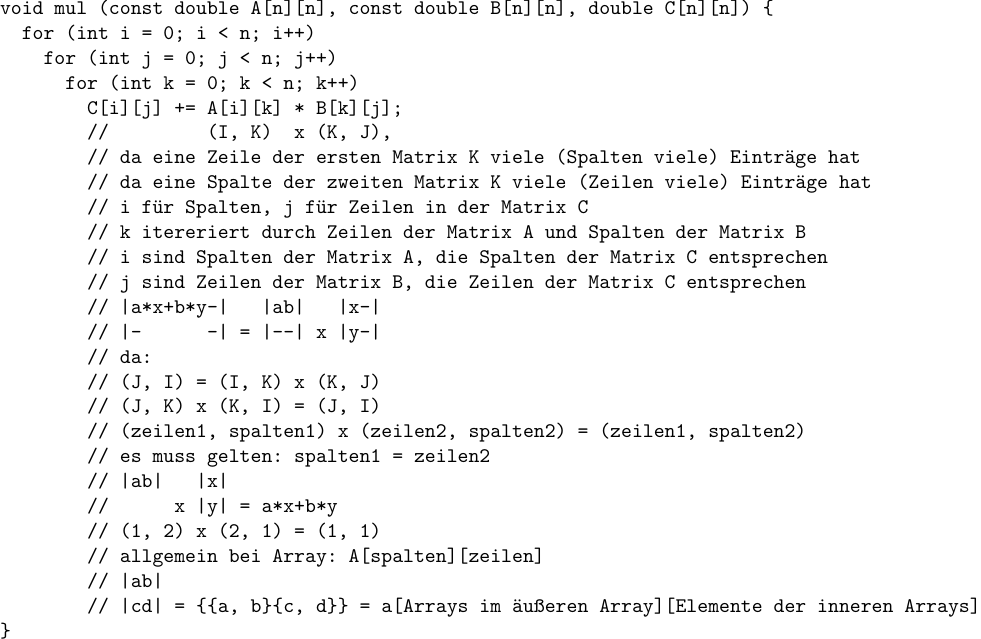
\includegraphics[width=\textwidth]{./figures/matrix_multiply.png}
              \end{minipage}
            }
          }
            child {
              node {Row- and Column-Major
                \resizebox{\textwidth}{!}{
                  \begin{minipage}[t]{8cm}
                    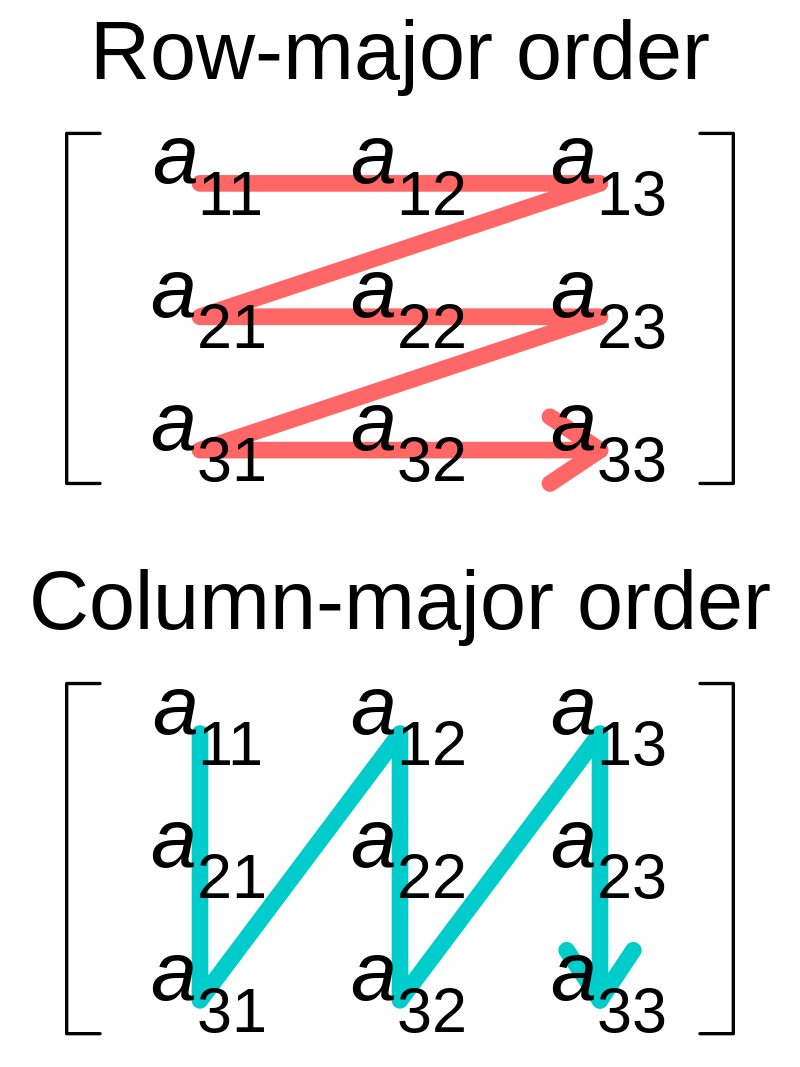
\includegraphics[width=0.3\textwidth, valign=t]{./figures/row_column_major.png} 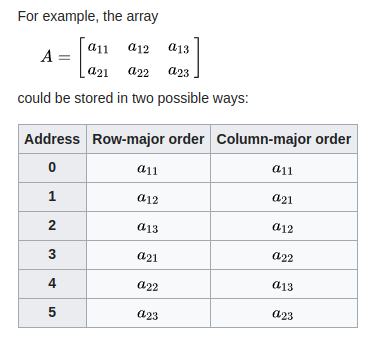
\includegraphics[width=0.7\textwidth, valign=t]{./figures/row_column_major_2.png}
                  \end{minipage}
                }
              }
            }
        }
        child {
          node {Conversion between different data units / systems
            \resizebox{\textwidth}{!}{
              \begin{minipage}[t]{8cm}
                \begin{itemize}
                  \item $Word \overset{\cdot 4}{\underset{/4}{>}} Byte \overset{\cdot 2}{\underset{/2}{>}} Hex \overset{\cdot 4}{\underset{/4}{>}} Bit$
                \end{itemize}
              \end{minipage}
            }
          }
        }
        child {
          node {Order of magnitude}
        }
        child {
          node {Endianes
            \resizebox{\textwidth}{!}{
              \begin{minipage}[t]{8cm}
                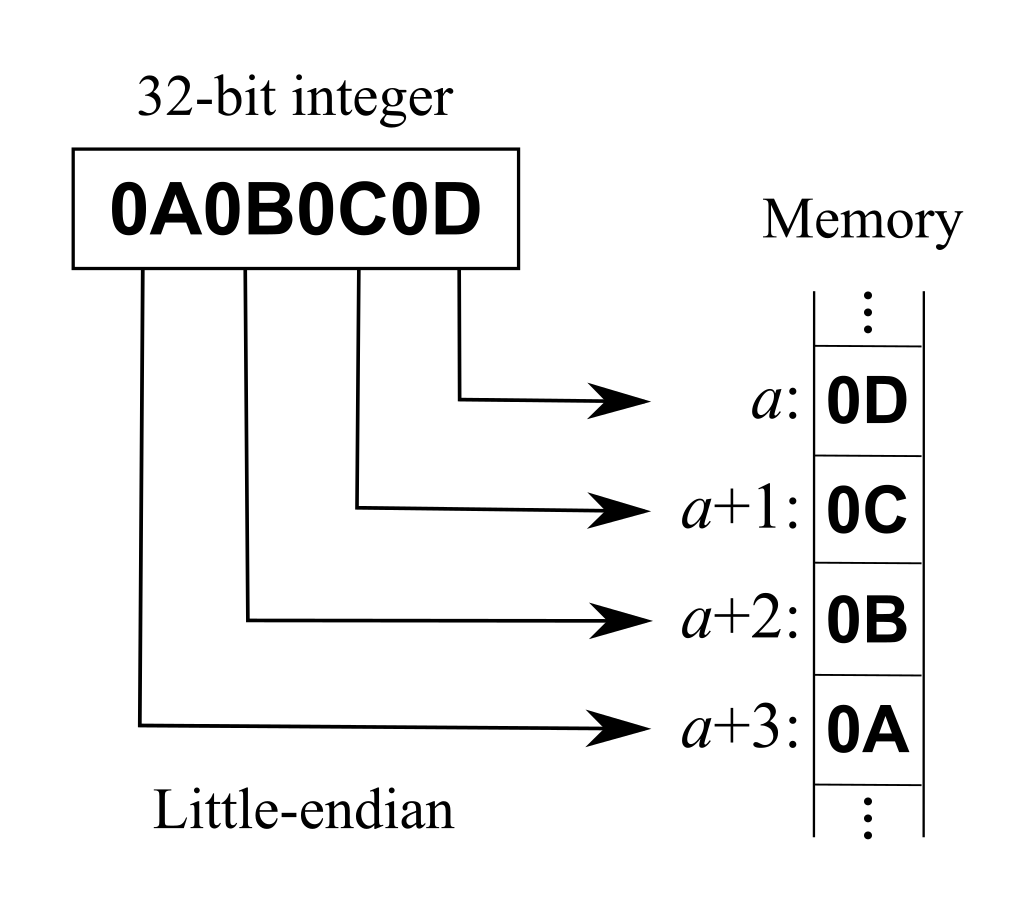
\includegraphics[width=0.5\textwidth, valign=t]{./figures/endianes.png}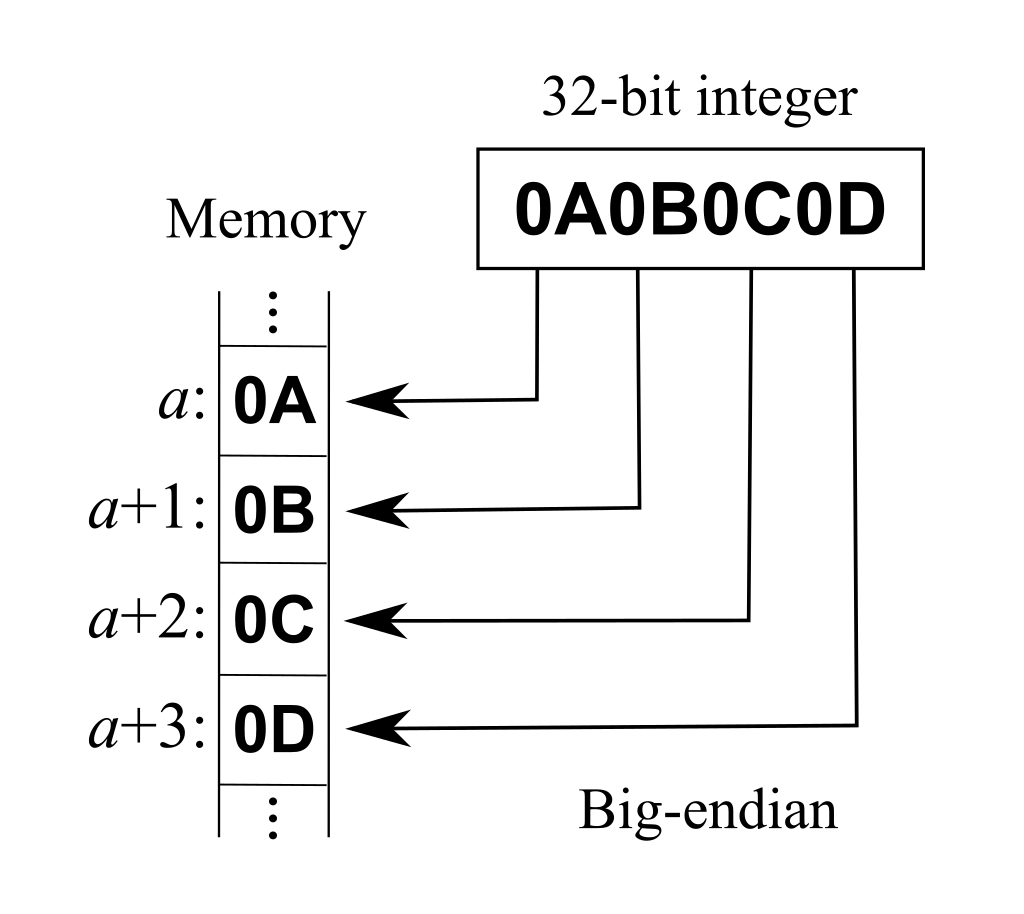
\includegraphics[width=0.5\textwidth, valign=t]{./figures/endianes_2.png}
              \end{minipage}
            }
          }
        }
        child {
          node {Design Principles}
            child {
              node {1. Simplicity favors regularity
                \resizebox{\textwidth}{!}{
                  \begin{minipage}[t]{8cm}
                    \begin{itemize}
                      \item Regularity makes implementation simpler
                      \item Simplicity enables higher performance at lower cost
                      % \item Make design more regular by simplifying the different variants and that allows to implement it faster
                    \end{itemize}
                  \end{minipage}
                }
              }
            }
            child {
              node {2. Smaller is faster
                \resizebox{\textwidth}{!}{
                  \begin{minipage}[t]{8cm}
                    \begin{itemize}
                      \item main memory: millions of locations
                    \end{itemize}
                  \end{minipage}
                }
              }
            }
            child {
              node {3. Good design demands good compromises
                \resizebox{\textwidth}{!}{
                  \begin{minipage}[t]{8cm}
                    \begin{itemize}
                      \item Different formats complicate decoding, but allow 32-bit instructions uniformly
                      \item Keep formats as similar as possible
                    \end{itemize}
                  \end{minipage}
                }
              }
            }
        }
        child {
          node {Seven Great Ideas}
            child {
              node {Use abstraction to simplify design}
            }
            child {
              node (commoncasefast) {Make the common case fast}
            }
            child {
              node {Performance via Parallelism}
            }
            child {
              node {Performance via Piplelining}
            }
            child {
              node {Performance via Prediction}
            }
            child {
              node {Hierarchy of Memories}
            }
            child {
              node {Dependability via Redundancy}
            }
        }
        child {
          node {Small Tricks}
            child {
              node {$\le$ and $<$
                \resizebox{\textwidth}{!}{
                  \begin{minipage}[t]{8cm}
                    \begin{itemize}
                      \item $x\le 2 \Leftrightarrow x < 2+1$:\\[0.25cm]
                        \begin{tabular}{c|c|c|c|c}
                          0 & 1 & 2 & 3 & 4 \\
                          \hline
                            &   & $\le$ & \textless &   \\
                          \hline
                          x & x & x &   &   \\
                      \end{tabular}
                      \item $x\ge 2 \Leftrightarrow x > 2-1$:\\[0.25cm]
                        \begin{tabular}{c|c|c|c|c}
                          0 & 1 & 2 & 3 & 4 \\
                          \hline
                            & \textgreater & $\ge$ &  &  \\
                          \hline
                            &   & x & x & x \\
                      \end{tabular}
                    \end{itemize}
                  \end{minipage}
                }
              }
            }
            child {
              node {Schnelles Prozentrechnen
                \resizebox{\textwidth}{!}{
                  \begin{minipage}[t]{8cm}
                    \begin{itemize}
                      \item $0.8 \cdot 20 = \frac{0.8 \cdot 10 \cdot 20}{10} = \frac{8 \cdot 20}{10} = \frac{160}{10} = 16$
                      \item $0.02 \cdot 20 = \frac{0.02 \cdot 100 \cdot 20}{100} = \frac{2 \cdot 20}{100} = 0.4$
                    \end{itemize}
                  \end{minipage}
                }
              }
            }
            child {
              node {Frequenzrechnung
                \resizebox{\textwidth}{!}{
                  \begin{minipage}[t]{8cm}
                    \begin{itemize}
                      \item Invertiert bekommt man Zeitdauer für ein Ereignis, da $f=\frac{N}{T} \Leftrightarrow T=\frac{N}{f}$ und $T_1=\frac{1}{f}$ und $T_2 = 2 \cdot \frac{1}{F}$
                      % bzw. zwischen dem Ende des betrachteten Ereignisses und dem Endes des letzten Ereignisses
                      \begin{itemize}
                        \item Frequenz ist immer wie oft sich eine Sache pro Zeiteinheit wiederholt wird ($Hz=\frac{1}{s}$)
                      \end{itemize}
                    \end{itemize}
                  \end{minipage}
                }
              }
            }
            child {
              node {Fraction Tricks
                \resizebox{\textwidth}{!}{
                  \begin{minipage}[t]{8cm}
                    \begin{itemize}
                      \item kürzen
                    \end{itemize}
                  \end{minipage}
                }
              }
          }
          child {
            node {Schnell Gleichungen umstellen}
          }
        }
    }
    child {
      node (performance) {Measuring Performance
        \resizebox{\textwidth}{!}{
          \begin{minipage}[t]{13cm}
            \begin{itemize}
              \item \alert{Define Performance:} $\displaystyle \frac{1}{Execution\;Time}$
              \item \alert{Relative Performance / Speedup:} \enquote{$X$ is $n$ times faster than $Y$} or \enquote{$Y$ is $n$ times slower than $X$}:\\[0.25cm] $\displaystyle \frac{Performance_X}{Performance_Y} = \frac{Execution\;Time_Y}{Execution\;Time_X} = n$
              \item \alert{Improved by:}
                \begin{itemize}
                  \item Reducing number of clock cycles
                  \item Increasing clock rate
                  \item trade off: higher clock rate vs. cycle count
                \end{itemize}
              \item \alert{Depends on:}
                \begin{itemize}
                  \item Algorithm (affects $IC$, possibly $CPI$)
                  \item Programming Language (affects $IC$, $CPI$)
                  \item Compiler (affects $IC$, $CPI$)
                  \item ISA (affects $IC$, $CPI$, $T_C$)
                \end{itemize}
            \end{itemize}
          \end{minipage}
        }
      }
      child {
        node {Power Benchmarks}
          child {
            node {SPEC Power Benchmark}
          }
          child {
            node {i7 Power Benchmark}
          }
      }
      child {
        node (measuringexecutiontime) {Measuring Execution Time}
          child {
            node (elapsedtime) {Elapsed Time}
          }
          child {
            node (cputime) {CPU Time
              \resizebox{\textwidth}{!}{
                \begin{minipage}[t]{8cm}
                  \begin{itemize}
                    \item $\begin{aligned}[t]
                        \displaystyle CPU\;Time&=Clock\;Cycles\times Clock\;Cycle\;Time\\
                                                    &=\frac{Clock\;Cycles}{Clock\;Rate} % \\
                                                    % &=\frac{Clock\;Cycles}{Instruction}
                                                    % =\frac{Instructions}{Program}
                                                    % =\frac{Seconds}{Clock\;Cycle}
                      \end{aligned}$
                    \item $\begin{aligned}[t]Clock\;Cycles &= Instruction\;Count\times CPI\\
                    &(CPI = Cycles\;per\;Instruction)\\
                    &=\sum^{n}_{i=1}\left(CPI_i\times Instruction\;Count_i\right)\\
                    &(\text{if different instruction classes take}\\&\text{different different number of cycles})\end{aligned}$
                    \item \alert{Weighed average CPI:}\\[0.25cm]$\displaystyle\begin{aligned} CPI = \frac{Clock\;Cycles}{Instruction\;Count}=\sum^{n}_{i=1}\left(CPI_i\times \frac{Instruction\;Count_i}{Instruction\;Count} \right)\end{aligned}$
                    \item $\displaystyle IPC = \frac{Instruction\;Count}{Clock\;Cycles}$
                    \begin{itemize}
                      \item Some designers invert CPI to talk about IPC, or instructions per clock cycle. If a processor executes on average two instructions per clock cycle, then it has an IPC of 2 and hence a CPI of 0.5
                    \end{itemize}
                  \end{itemize}
                \end{minipage}
              }
            }
              child {
                node (speccpubenchmark) {SPEC CPU Benchmark
                  \resizebox{\textwidth}{!}{
                    \begin{minipage}[t]{8cm}
                      \begin{itemize}
                        \item $\displaystyle \sqrt[n]{\prod^{n}_{i=1} Execution\;Time\;Ratio_i}$
                      \end{itemize}
                    \end{minipage}
                  }
                }
              }
          }
      }
      child {
        node {\alert{Ticks} (Cache line excesses) and \alert{MEMS} (how many memory accesses it does)}
      }
      child {
        node {Clock Cycles}
      }
      child {
        node (amdahl) {Amdahl's Law
          \resizebox{\textwidth}{!}{
            \begin{minipage}[t]{9cm}
              \begin{itemize}
                \item \alert{Improving an aspect} of a computer and expecting a proportional improvement in \alert{overall performance}
                \item $\displaystyle T_{improved} = \frac{T_{affected}}{improvement\;factor} + T_{unaffected}$
                \item \alert{how fast with $p$ cores?}: $t_1 = 100s$, $t_2 = 90s$, $u_1 + \frac{u_2}{p} = t_p$, $\frac{u_2}{p} = t_1 - t_p \Leftrightarrow \frac{u_2}{2}  = 10 \Leftrightarrow u_2 = 20$, \alert{4 Cores:} $80 + \frac{20}{4} = 85s$
              \end{itemize}
            \end{minipage}
          }
        }
      }
    }
    child {
      node {Integer Arithmetic}
        child {
          node {2's Complement}
            child {
              node {Biggest 2's Complement Negative Number}
            }
        }
        child {
          node {Verification
            \resizebox{\textwidth}{!}{
              \begin{minipage}[t]{8cm}
                \begin{itemize}
                  \item set up a input equation $e_1$ how input bits should be calulcated together arithmetically
                  \item set up a output equation $e_2$ with the intented output bits that is equal to $e_1$
                  \item start at the output equation $e_2$ to translate to polynomial ring modulo 2 and try to get equation $e_1$ again
                \end{itemize}
              \end{minipage}
            }
          }
            child {
              node {Polynomial Ring Modulo 2
                \resizebox{\textwidth}{!}{
                  \begin{minipage}[t]{8cm}
                    \begin{itemize}
                      \item \alert{Rules:}
                      \begin{itemize}
                        \item $a\wedge b \equiv a\cdot b$
                        \item $a\vee b \equiv a+b - a\cdot b$
                        \item $a\oplus b \equiv a+b - 2\cdot a\cdot b$
                        \item $\neg a \equiv 1-a$
                        \item $a^2 \equiv a$ (Modulo 2)
                      \end{itemize}
                    \end{itemize}
                  \end{minipage}
                }
              }
            }
        }
        child {
          node {Circuits}
            child {
              node {AND-Inverter-Graph (AIG)
                \resizebox{\textwidth}{!}{
                  \begin{minipage}[t]{8cm}
                    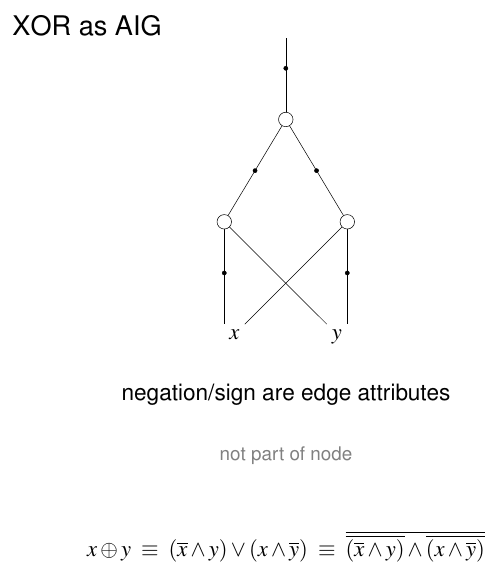
\includegraphics[width=\textwidth]{./figures/aig.png}
                  \end{minipage}
                }
              }
            }
            child {
              node {Amdahls Law with Work and Span
                \resizebox{\textwidth}{!}{
                  \begin{minipage}[t]{8cm}
                    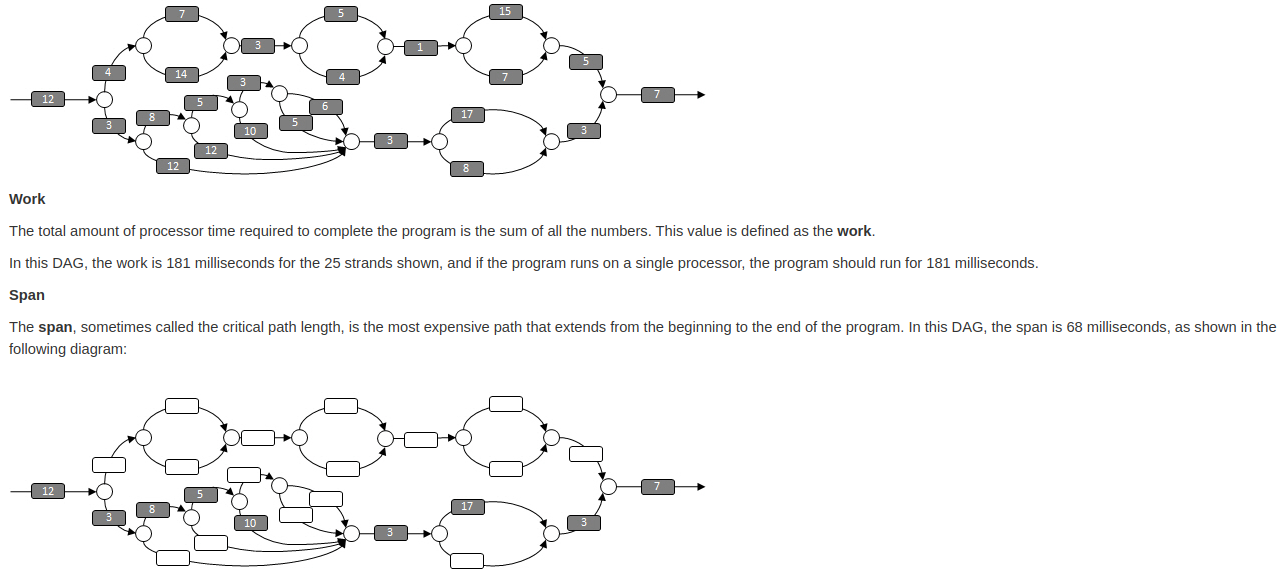
\includegraphics[width=\textwidth]{./figures/work_span_2.png}
                    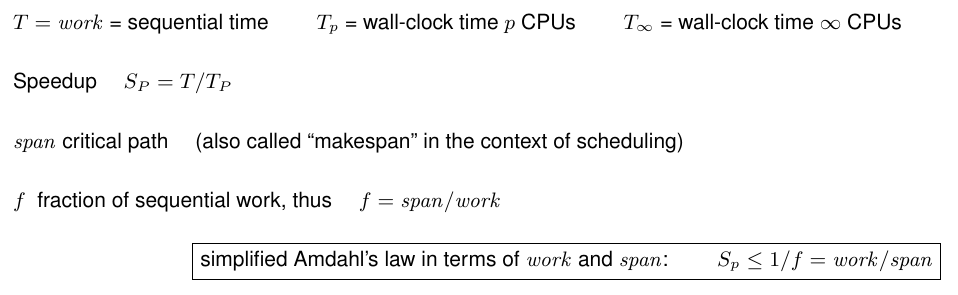
\includegraphics[width=\textwidth]{./figures/work_span_slides.png}
                  \end{minipage}
                }
              }
            }
            child {
              node {Multiplexer}
            }
            child {
              node {Adders}
                child {
                  node {Half Adder and Full Adder
                    \resizebox{\textwidth}{!}{
                      \begin{minipage}[t]{12cm}
                        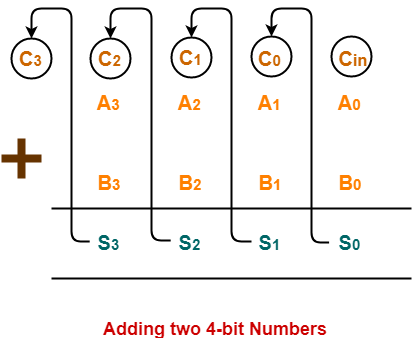
\includegraphics[width=\textwidth]{./figures/addition.png}
                        \begin{itemize}
                          \item das ist einfach nur die Umsetzung von a+b+ci oben und beide Möglichkeiten wie ein Übertrag enstehen kann müssen entsprechend behandelt werden
                          \item ob die beiden Überträge am Ende gexort oder geort werden spielt keine Rolle, da es sowieso niemals vorkommen kann, dass beide HA einen Übertrag haben
                          \begin{itemize}
                            \item beim zweiten HA kommt es zu einem Übertrag, wenn s0 und ci beide 1 sind
                            \item beim ersten HA kommt es zu einem Übertrag, wenn a und b beide 1 sind
                            \item wenn der erste HA einen Übertrag hat, bedeutet es für den zweiten, dass s0 0 sein muss es somit beim zweiten zu keinem Übertrag kommen kann
                            \item wenn der zweite HA einen Übertrag hat, bedeutet es für den ersten, dass bei diesem s0 1 ist und es dafür keinen Übertrag haben kann. Bei HA kann es nicht vorkommen, dass co0s0=11
                          \end{itemize}
                        \end{itemize}
                        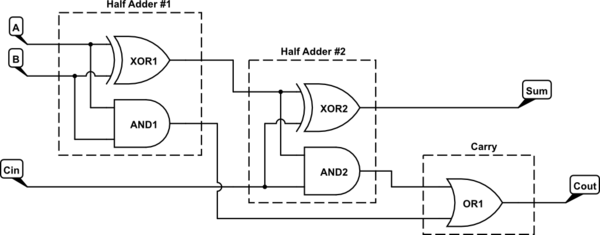
\includegraphics[width=\textwidth]{./figures/HA_and_FA.png}
                        \begin{itemize}
                         \item es spielt bei FA bei der Verwendung keine Rolle, welches der 3 Inputs eigentlich für das Carry vorgesehen ist
                        \end{itemize}
                        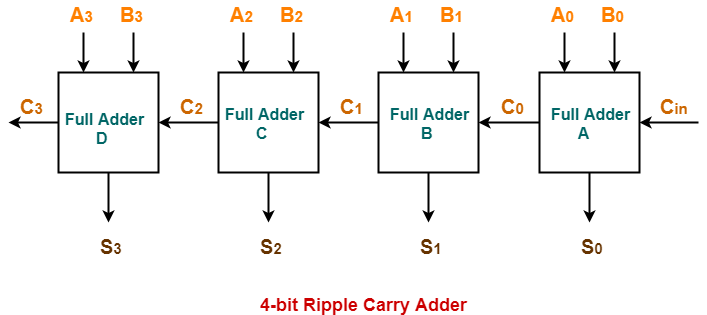
\includegraphics[width=\textwidth]{./figures/4_adder_substractor.png}
                        \begin{itemize}
                          \item der FA kann 3 Inputs zusammenrechnen, daher sind die möglichen Outputs 00 01 10 11
                          \item der HA kann 2 Inputs zusammenrechen, daher sind die möglichen Outputs 00 01 10
                          \item angeordnet werden sie in einem 4-Bit Addierer als:
                          \begin{itemize}
                            \item FA FA FA HA, wobei man allerdings meistens FA FA FA FA herstellt und das carry vom letzten FA unberührt lässt, sodass man Addierer zu größeren Addierern stacken kann
                          \end{itemize}
                        \end{itemize}
                      \end{minipage}
                    }
                  }
                }
                child {
                  node {Determine overflow with carry-in and carry-out of the MSB
                    \resizebox{\textwidth}{!}{
                      \begin{minipage}[t]{8cm}
                        \begin{itemize}
                          \item An overflow is the case if and only if the carry-in and carry-out of the most significant bit are not equal.
                          \item $a+b$
                          \begin{itemize}
                             \item \alert{Case 1:} $a \ge 0$ and $b \ge 0$: both MSB are $0$, so carry-out has to be $0$, a carry-in of $1$ would make the number negative
                             \item \alert{Case 2:} $a < 0$ and $b < 0$: both MSB are $1$, so carry-out has to be $1$, a carry-in of $0$ would make the number positive as addition of the two MSB's results in $01_2 + 01_2 = 10_2$ and only a carry-in of $1$ would let the number stay negative, i.e. let the MSB of the resulting number stay $1$: $01_2 + 01_2 + 01_2 = 11_2$.
                             \item \alert{Case 3:} $a \ge 0$ and $b < 0$ or $a < 0$ and $b \ge 0$: one MSB is $0$ and the other one is $1$, carry-out will be $0$. No Overflow possible by adding a positve and a negative number, so carry-in will also be $0$
                          \end{itemize}
                          \item $a-b$:
                          \begin{itemize}
                            \item $a \ge 0$ and $b \ge$: same as Case 3
                            \item $a < 0$ and $b < 0$: same as Case 3
                            \item $a \ge 0$ and $b < 0$: same as Case 1
                            \item $a < 0$ and $b \ge 0$: same as Case 2
                          \end{itemize}
                        \end{itemize}
                      \end{minipage}
                    }
                  }
                }
                child {
                  node {Ripple-Carry-Adder
                    \resizebox{\textwidth}{!}{
                      \begin{minipage}[t]{8cm}
                        \begin{itemize}
                          \item \alert{work:} $n$
                          \item \alert{span:} $n$
                        \end{itemize}
                        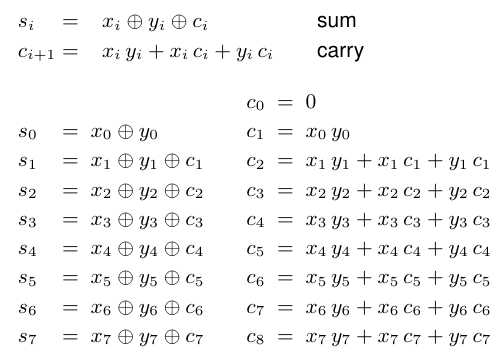
\includegraphics[width=\textwidth]{./figures/rippel_carry_adder.png}
                      \end{minipage}
                    }
                  }
                  child {
                    node {Prefix Sum / Scan
                      \resizebox{\textwidth}{!}{
                        \begin{minipage}[t]{8cm}
                          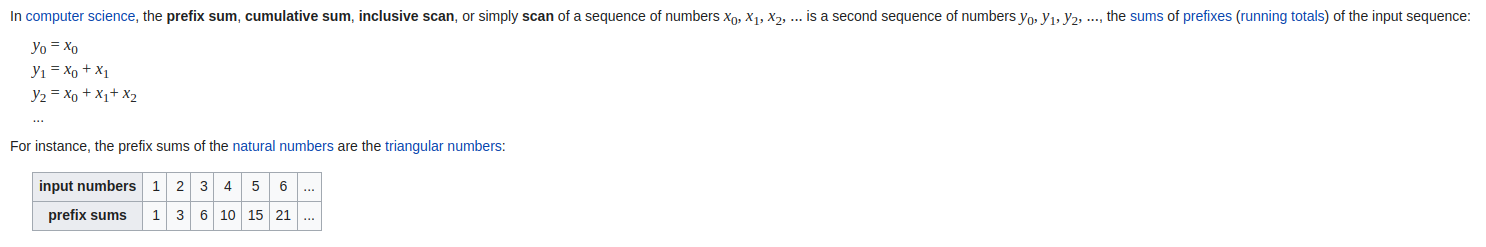
\includegraphics[width=\textwidth]{./figures/prefix_sum.png}
                          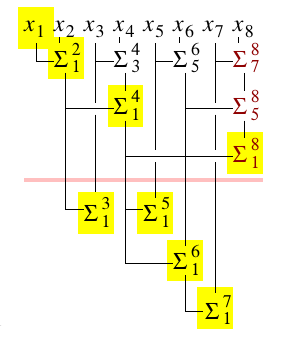
\includegraphics[width=0.25\textwidth]{./figures/scan.png}
                        \end{minipage}
                      }
                    }
                  }
                }
                % child {
                %   node {Propagate-and-Generate Adder / Lookahead Adder
                %     \resizebox{\textwidth}{!}{
                %       \begin{minipage}[t]{8cm}
                %         \begin{itemize}
                %           \item using prefix / scan computation
                %         \end{itemize}
                %       \end{minipage}
                %     }
                %   }
                % }
                child {
                  node {Carry-Lookahead Adder
                    \resizebox{\textwidth}{!}{
                      \begin{minipage}[t]{8cm}
                        \begin{itemize}
                          \item \alert{work:} $n^2$
                          \item \alert{span:} $log(n)$
                        \end{itemize}
                      \end{minipage}
                    }
                  }
                  child {
                    node {Propagate and Generate
                      \resizebox{\textwidth}{!}{
                        \begin{minipage}[t]{8cm}
                          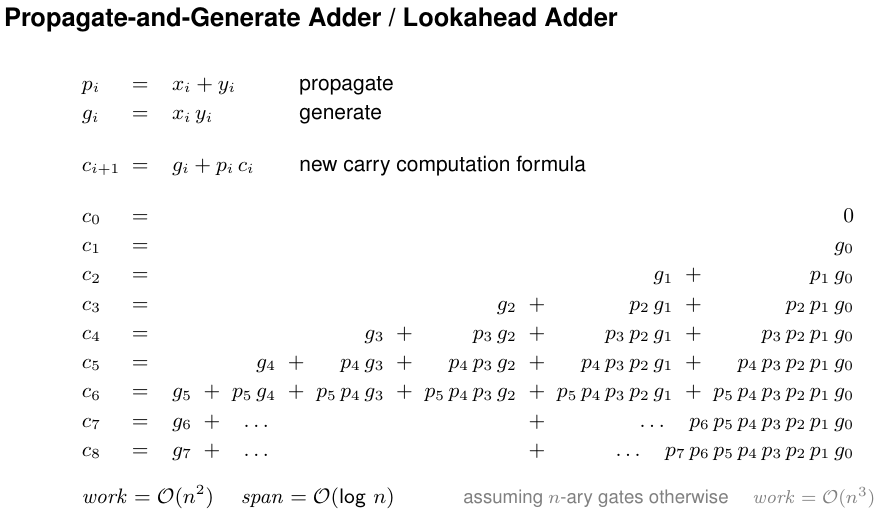
\includegraphics[width=\textwidth]{./figures/propagate_and_generate.png}
                        \end{minipage}
                      }
                    }
                  }
                }
            }
            child {
              node {Multipliers
                \resizebox{\textwidth}{!}{
                  \begin{minipage}[t]{8cm}
                    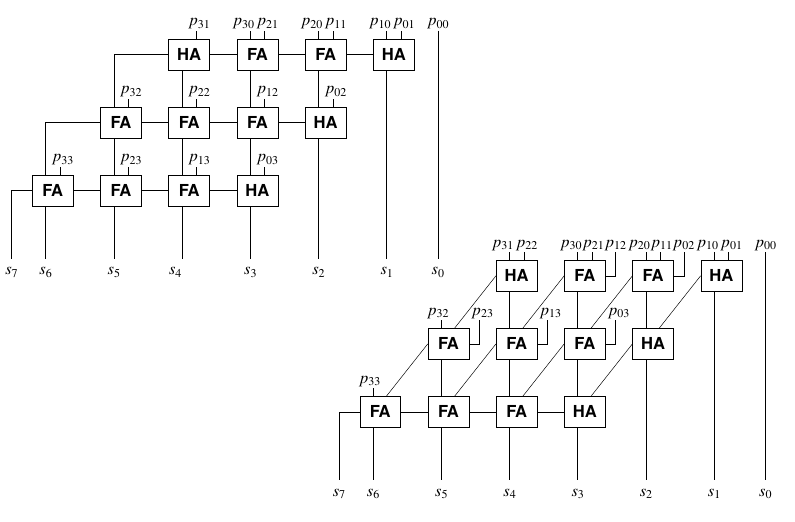
\includegraphics[width=\textwidth]{./figures/multipliers.png}
                  \end{minipage}
                }
              }
                child {
                  node {Multplication with rational numbers}
                }
                child {
                  node {Array Ripple Carry Multiplier}
                }
                child {
                  node {Wallace-Tree Carry-Lookahead Multiplier}
                  child {
                    node {Wallace-Tree
                      \resizebox{\textwidth}{!}{
                        \begin{minipage}[t]{8cm}
                          \begin{itemize}
                            \item A Wallace multiplier is a hardware implementation of a binary multiplier, a digital circuit that multiplies two integers. It uses a selection of full and half adders (the Wallace tree or Wallace reduction) to sum partial products in stages until two numbers are left. Wallace multipliers reduce as much as possible on each layer %, whereas Dadda multipliers try to minimize the required number of gates by postponing the reduction to the upper layers
                          \end{itemize}
                        \end{minipage}
                      }
                    }
                  }
                }
                child {
                  node {Binary Multiplication
                    \resizebox{\textwidth}{!}{
                      \begin{minipage}[t]{8cm}
                        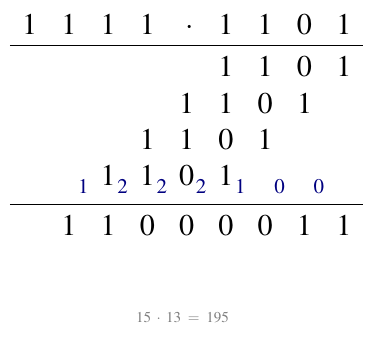
\includegraphics[width=\textwidth]{./figures/multiplication.png}
                      \end{minipage}
                    }
                  }
                }
            }
            child {
              node {Comparison
                \resizebox{\textwidth}{!}{
                  \begin{minipage}[t]{8cm}
                    \begin{itemize}
                      \item \alert{Equality}: $\displaystyle \bigwedge_{i=0}^{31} \neg(x_i\oplus y_i)$
                      \begin{itemize}
                        \item comporison constant and log(n) and's needed
                      \end{itemize}
                      \item \alert{Greater}: $x[31\ldots 0] > y[31\ldots 0] \Leftrightarrow x_{31}\overline{y_{31}} \vee x_{31}={y_{31}}\cdot (x[30\ldots 0] > y[30\ldots 0])$
                      \begin{itemize}
                        \item linear latency $n$ (do substraction and then compare to $0$), more space in hardware and time than Equality. Equality is faster and less hardware
                      \end{itemize}
                      \item \alert{Greater Equals}: $x[31\ldots 0] \ge y[31\ldots 0] \Leftrightarrow x_{31}\overline{y_{31}} \vee x_{31}={y_{31}}\cdot (x[30\ldots 0] > y[30\ldots 0]) \vee x_0 = y_0$
                      \item don't want to slow down stages of pipeline and don't want to inrease size of cpu too much in this stage for second ALU
                    \end{itemize}
                  \end{minipage}
                }
              }
            }
            child {
              node {Barrel Shifter}
            }
            child {
              node {Decoder}
            }
        }
    }
    child {
      node {Floating Point Arithmetic
        \resizebox{\textwidth}{!}{
          \begin{minipage}[t]{14cm}
            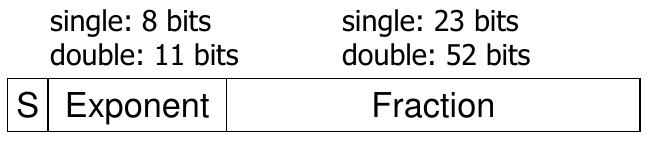
\includegraphics[width=\textwidth]{./figures/floating_point.png}
            \begin{itemize}
              \item $encoded\_exponent = real\_exponent + bias$
              \item $real\_exponent = encoded\_exponent - bias$
              \item $significand = 1 + fraction$
              \item calculations are always made with $real\_exponent$
              \item the bias that makes the \alert{exponent} always \alert{positive} and the ordering that the expontent is coming before the \alert{fraction/mantissa} is only there so such that one can efficiently compare floating point numbers which one is bigger etc.
              \item \alert{Floating point} numbers has a varying number of digits after the decimal point. \alert{Fixed point} numbers have a fixed number of digits after the decimal point and by this a smaller representation range than floating point numbers. In the floating point system the numbers \alert{aren't equaly distributed}, one has a very \alert{high density of small numbers} close to 0, besides a very small section close to 0 with no numbers at all.
              \item there are \alert{special registers} for \alert{floating point} because one wants to have \alert{floating points registers} close to the **floating point unit** and \alert{integer registers} close to the general \alert{ALU} and wire lenghts matter as getting a signal along a wire takes time.
            \end{itemize}
          \end{minipage}
        }
      }
      child {
        node {Formats}
          child {
            node {Bfloat8
              \resizebox{\textwidth}{!}{
                \begin{minipage}[t]{8cm}
                  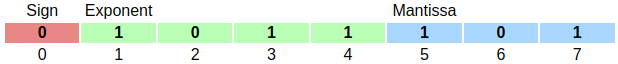
\includegraphics[width=\textwidth]{./figures/bfloat8.png}
                \end{minipage}
              }
            }
          }
      }
      child {
        node {Arithmetic}
          child {
            node {Addition
              \resizebox{\textwidth}{!}{
                \begin{minipage}[t]{8cm}
                  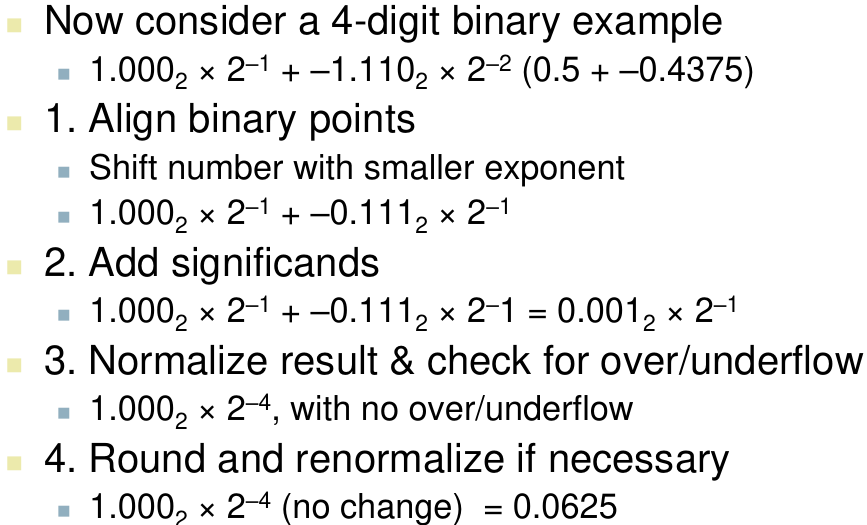
\includegraphics[width=\textwidth]{./figures/floating_point_addition.png}
                  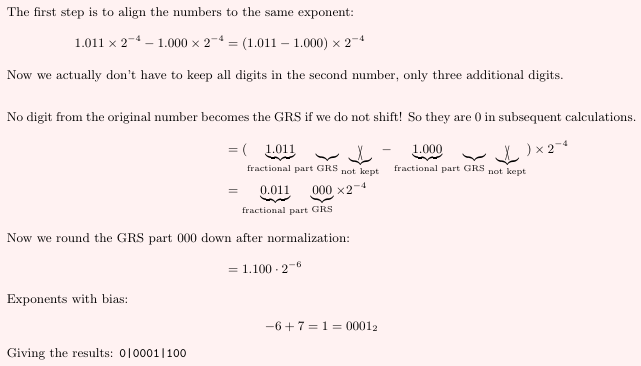
\includegraphics[width=0.5\textwidth, valign=t]{./figures/floating_point_addition_example.png}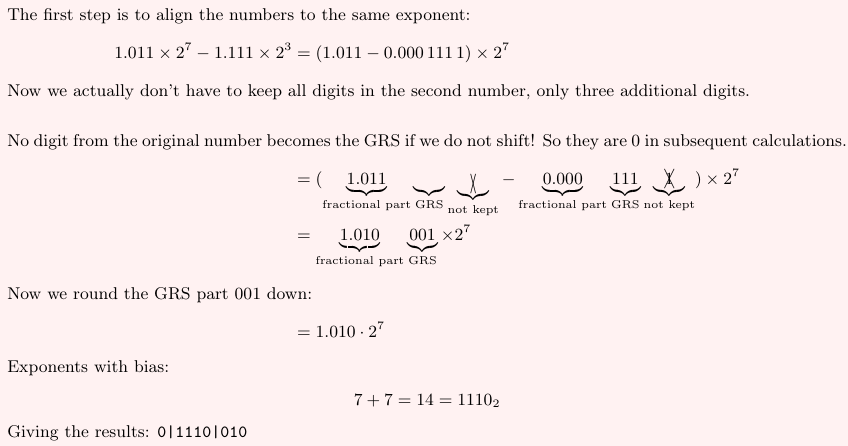
\includegraphics[width=0.5\textwidth, valign=t]{./figures/floating_point_addition_example_2.png}
                \end{minipage}
              }
            }
          }
          child {
            node {Multiplication
              \resizebox{\textwidth}{!}{
                \begin{minipage}[t]{8cm}
                  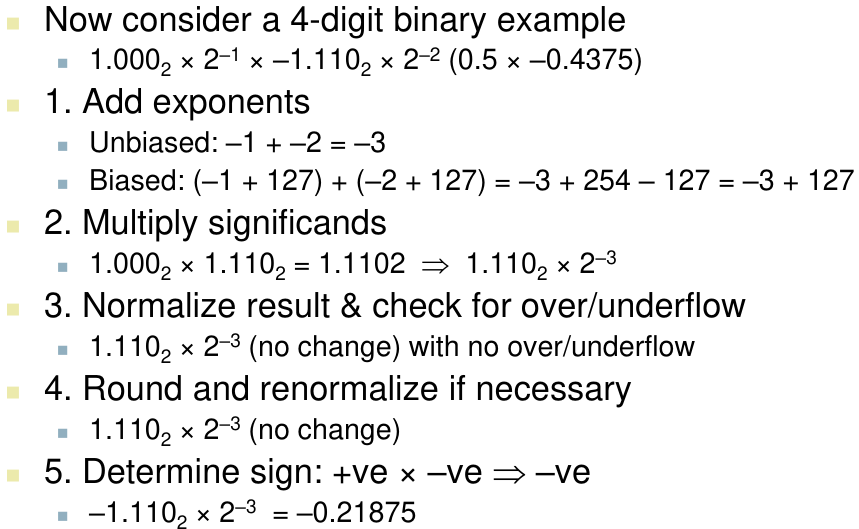
\includegraphics[width=\textwidth]{./figures/floating_point_multiplication.png}
                \end{minipage}
              }
            }
          }
      }
      child {
        node {Types of Numbers}
          child {
            node {Normalised Numbers
              \resizebox{\textwidth}{!}{
                \begin{minipage}[t]{11cm}
                  \begin{itemize}
                    \item $x = ( -1)^S \times (1 + Fraction) \times 2^{Exponent - Bias}$, $\boxed{\frac{0}{1}\mid 1101\mid 010}$
                    \item $Bias = 2^{e-1} - 1$, 7, $\boxed{0111}$
                    \item \alert{Smallest normalised number} $\pm 1.125 \times 2^{1-7}$, $\boxed{\frac{0}{1}\mid 0001\mid 000}$
                    \item \alert{Largest normalised number} $\approx \pm 1.875 \times 2^{14-7}$, $\boxed{\frac{0}{1}\mid 1110\mid 111}$
                    \item \alert{Normalising:} $0.011 \cdot 2^2 \cdot \frac{2^{-4}}{2^2} = 1.100 \cdot 2^{-6}$
                  \end{itemize}
                \end{minipage}
              }
            }
          }
          child {
            node {Denormalised Numbers
              \resizebox{\textwidth}{!}{
                \begin{minipage}[t]{11cm}
                  \begin{itemize}
                    \item $x = ( -1)^S \times (0 + Fraction) \times 2^{-Bias}$, $\boxed{\frac{0}{1}\mid 0000\mid 010}$
                    \item $Bias = 2^{e-1} - 2$, 6, $\boxed{0110}$
                    \item \alert{Smallest denormalised number that is not $0$} $\pm 0.125 \times 2^{0-6}$, $\boxed{\frac{0}{1}\mid 0000\mid 001}$
                    \item \alert{Largest denormalised number} $\approx \pm 0.875 \times 2^{0-6}$, $\boxed{\frac{0}{1}\mid 0000\mid 111}$
                  \end{itemize}
                \end{minipage}
              }
            }
          }
          child {
            node {Zero, Infinity, NaN
              \resizebox{\textwidth}{!}{
                \begin{minipage}[t]{8cm}
                  \begin{itemize}
                    \item \alert{Zero:} $\boxed{\frac{0}{1}\mid 0000\mid 000}$
                    \item \alert{Infinity:} $\boxed{\frac{0}{1}\mid 1111\mid 000}$
                    \item \alert{NaN:} $\boxed{\frac{0}{1}\mid 1111\mid 010}$
                  \end{itemize}
                \end{minipage}
              }
            }
          }
      }
      child {
        node {Rounding}
          child {
            node {Rounding rules
              \resizebox{\textwidth}{!}{
                \begin{minipage}[t]{8cm}
                  \begin{itemize}
                    \item \alert{Ties to even:} numbers exactly in the middle between two integer numbers (\enquote{ties}) are rounded towards the even number\\[0.25cm]
                    $0.5 \to 0,\\
                    1.5 \to 2,\\
                    2.5 \to 2$
                  \end{itemize}
                \end{minipage}
              }
            }
          }
          child {
            node {GRS Bits
              \resizebox{\textwidth}{!}{
                \begin{minipage}[t]{8cm}
                  \begin{itemize}
                    \item \alert{Guard}, \alert{Round} and \alert{Sticky Bit}, the \alert{Sticky bit} is a OR for all remaining bits that don't fit in the representation
                    \item with GRS just need $3$ additional bits, so one only needs a smaller and faster adder with which one has to do the calculations\\[0.25cm]
                    \item without GRS would have to do calculation with all bits and round at the end
                      $\begin{tabular}{llll}
                          &     & 1/8 & 0.125 \\
                          & 1/4 &     & 0.25  \\
                          & 1/4 & 1/8 & 0.375 \\
                      1/2 &     &     & 0.5   \\
                      1/2 &     & 1/8 & 0.625 \\
                      1/2 & 1/4 &     & 0.75  \\
                      1/2 & 1/4 & 1/8 & 0.875\\
                      G   & R   & S   &
                    \end{tabular}$
                  \end{itemize}
                \end{minipage}
              }
            }
          }
      }
      child {
        node {Conversion}
          child {
            node {Floating Point to Decimal
              \resizebox{\textwidth}{!}{
                \begin{minipage}[t]{8cm}
                  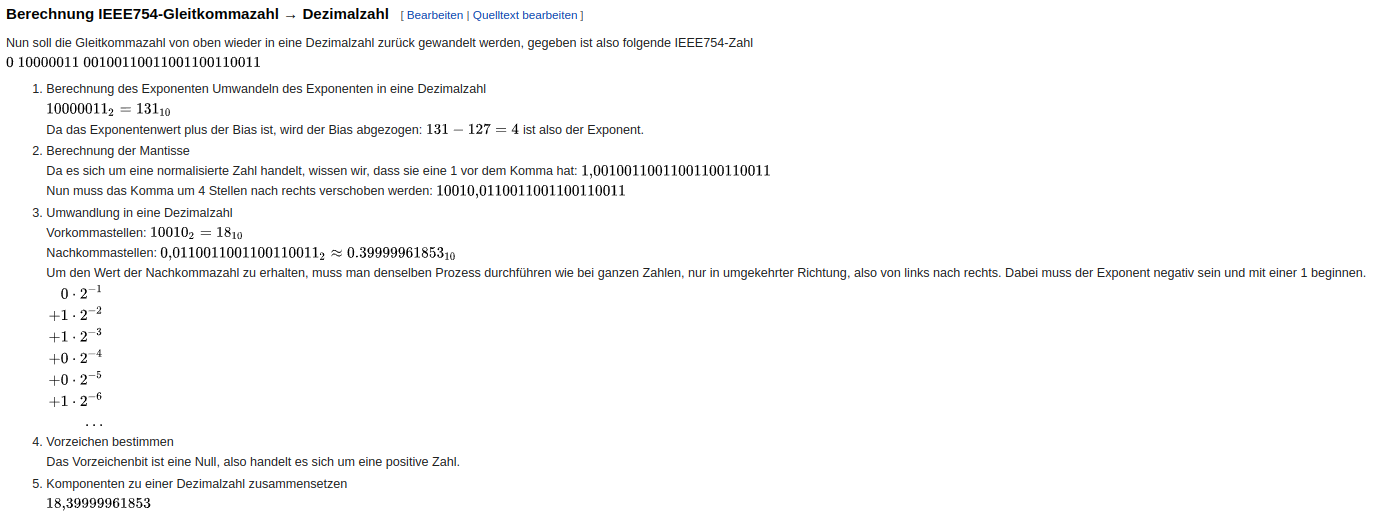
\includegraphics[width=\textwidth]{./figures/float_to_decimal.png}
                \end{minipage}
              }
            }
          }
          child {
            node {Decimal to Floating Point
              \resizebox{\textwidth}{!}{
                \begin{minipage}[t]{8cm}
                  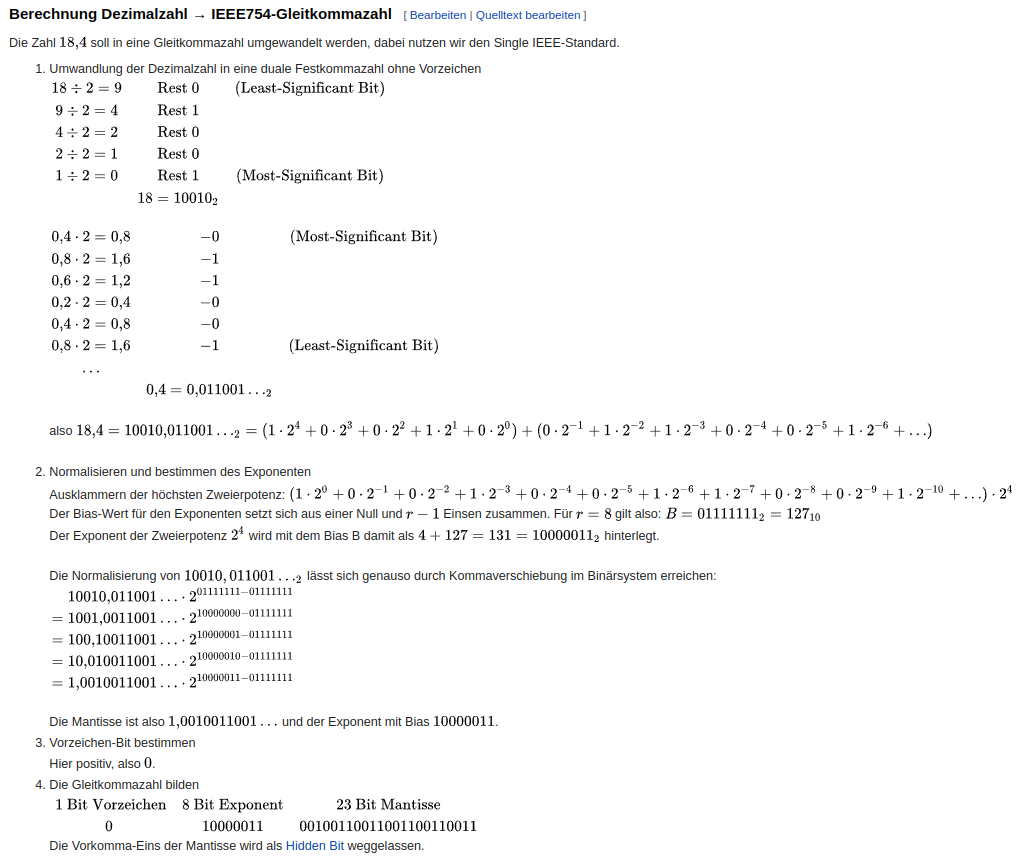
\includegraphics[width=\textwidth]{./figures/decicmal_to_float.png}
                \end{minipage}
              }
            }
          }
          child {
            node {Fraction
              \resizebox{\textwidth}{!}{
                \begin{minipage}[t]{8cm}
                  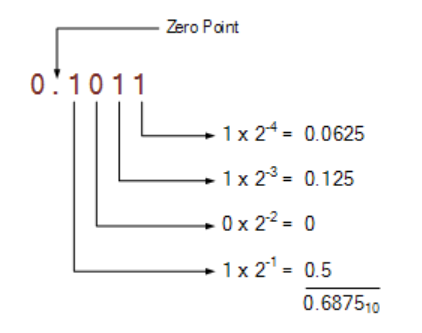
\includegraphics[width=0.5\textwidth]{./figures/binary_fraction.png} 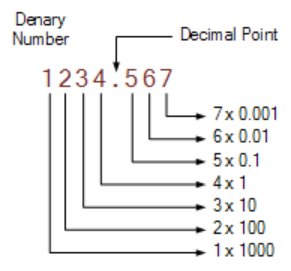
\includegraphics[width=0.5\textwidth]{./figures/decimal_fraction.png}
                \end{minipage}
              }
            }
          }
      }
    }
    child {
      node {Processor
        \resizebox{\textwidth}{!}{
          \begin{minipage}[t]{12cm}
            \begin{itemize}
              \item \alert{Control signal:} A signal used for multiplexor selection or for directing the operation of a functional unit
              \item \alert{Data signal:} Contains information that is operated on by a functional unit
              \item \alert{Datapath element:} A unit used to operate on or hold data within a processor. In the RISC-V implementation, the datapath elements include the instruction and data memories, the register
              \item \alert{Register file:} A state element that consists of a set of registers that can be read and written by supplying a register number to be accessed
              \item \alert{Control:} The component of the processor that commands the datapath, memory, and I/O devices according to the instructions of the program
            \end{itemize}
          \end{minipage}
        }
      }
        child {
          node {ISA
            \resizebox{\textwidth}{!}{
              \begin{minipage}[t]{8cm}
                \begin{itemize}
                  \item An abstract interface between the hardware and the lowest-level software that encompasses all the information necessary to write a machine language program that will run correctly, including instructions, registers, memory access, I/O, and so on
                \end{itemize}
              \end{minipage}
            }
          }
            child {
              node {Translation
                \resizebox{\textwidth}{!}{
                  \begin{minipage}[t]{8cm}
                    \begin{itemize}
                      \item \alert{Opcode:} The field that denotes the operation and format of an instruction.
                      \item \alert{Application binary Interface (ABI):} The user portion of the instruction set plus the operating system interfaces used by application programmers. It defines a standard for binary portability across computers
                    \end{itemize}
                  \end{minipage}
                }
              } [counterclockwise from=300] % https://tex.stackexchange.com/questions/118601/mindmap-sibling-angle-in-tikz
              child {
                node {If
                  \resizebox{\textwidth}{!}{
                    \begin{minipage}[t]{8cm}
                      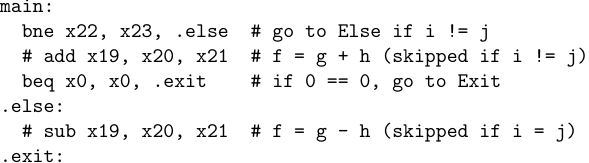
\includegraphics[width=\textwidth]{./figures/code_if.png}
                    \end{minipage}
                  }
                }
              }
              child {
                node {While
                  \resizebox{\textwidth}{!}{
                    \begin{minipage}[t]{8cm}
                      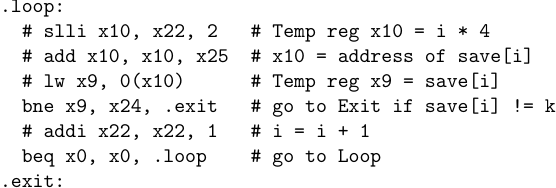
\includegraphics[width=\textwidth]{./figures/code_while.png}
                    \end{minipage}
                  }
                }
              }
              child {
                node {Function}
                  child {
                    node {With Framepointer
                      \resizebox{\textwidth}{!}{
                        \begin{minipage}[t]{8cm}
                          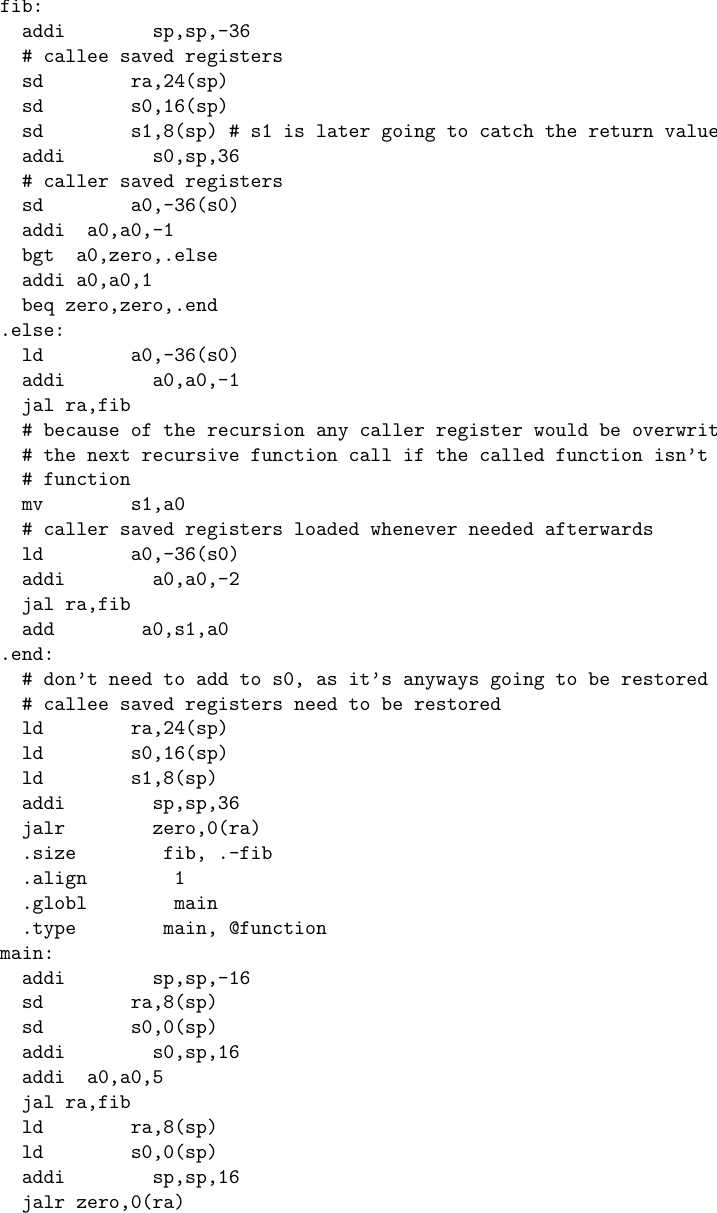
\includegraphics[width=\textwidth]{./figures/code_function_v2.png}
                        \end{minipage}
                      }
                    }
                  }
                  child {
                    node {Without Framepointer
                      \resizebox{\textwidth}{!}{
                        \begin{minipage}[t]{8cm}
                          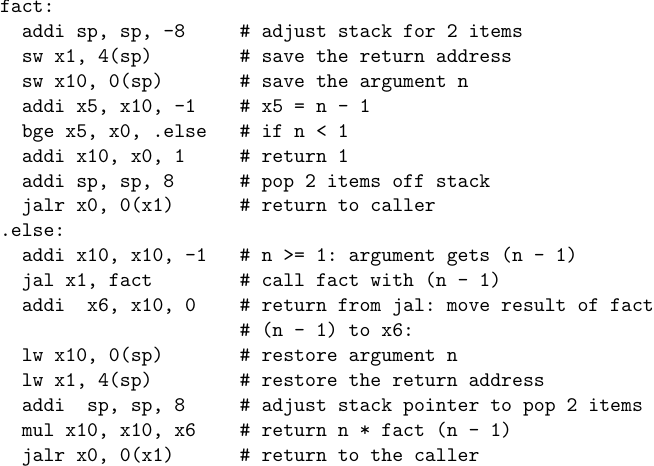
\includegraphics[width=\textwidth]{./figures/code_function_v1.png}
                        \end{minipage}
                      }
                    }
                  }
              }
              child {
                node {Array
                  \resizebox{\textwidth}{!}{
                    \begin{minipage}[t]{8cm}
                      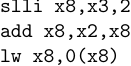
\includegraphics[width=0.3\textwidth]{./figures/code_array_2.png}\\[0.25cm]
                      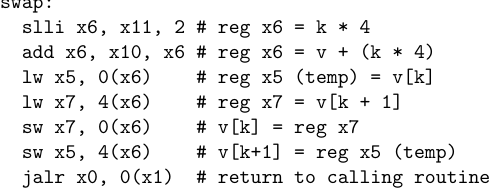
\includegraphics[width=\textwidth]{./figures/code_array.png}
                    \end{minipage}
                  }
                }
              }
            }
        }
        child {
          node {Exception
            \resizebox{\textwidth}{!}{
              \begin{minipage}[t]{8cm}
                \begin{itemize}
                  \item An unscheduled event that disrupts program execution
                  \item Some architectures use the term interrupt for all exceptions
                  \item Insert a breakpoint amounts to insert an exception that is caught by system instructions. Therefore the instrutions are changed.
                  \begin{itemize}
                    \item When the exception is raised, the normal flow is stopped (interrupting the pipeline and aborting instructions) and a system call is triggered.
                  \end{itemize}
                \end{itemize}
              \end{minipage}
            }
          }
            child {
              node {Handling Exceptions
                \resizebox{\textwidth}{!}{
                  \begin{minipage}[t]{10cm}
                    \begin{itemize}
                      \item Save PC of offending (or interrupted) instruction
                      \begin{itemize}
                         \item \alert{In RISC-V:} Supervisor Exception Program Counter (SEPC), register used to hold the address of the affected instruction. Such a register is needed even when exceptions are vectored
                      \end{itemize}
                      \item Save indication of the problem
                      \begin{itemize}
                        \item \alert{In RISC-V:} Supervisor Exception Cause Register (SCAUSE), used to record the cause of the exception
                      \end{itemize}
                      \item Jump to handler
                      \item After performing whatever action is required because of the exception, the operating system can terminate the program or may continue its execution, using the SEPC
                    \end{itemize}
                  \end{minipage}
                }
              }
                child {
                  node {Use of special register
                    \resizebox{\textwidth}{!}{
                      \begin{minipage}[t]{10cm}
                        \begin{itemize}
                          \item Include a register which holds a field that indicates the reason for the exception
                          \item Transfer control to the operating system at some specified address
                          \item Method used in the RISC-V architecture
                        \end{itemize}
                      \end{minipage}
                    }
                  }
                }
                child {
                  node {Vectored interrupt
                    \resizebox{\textwidth}{!}{
                      \begin{minipage}[t]{10cm}
                        \begin{itemize}
                          \item An interrupt for which the address to which control is transferred is determined by the cause of the exception
                          \item Possibly added to a base register that points to memory range for vectored interrupts
                        \end{itemize}
                      \end{minipage}
                    }
                  }
                }
            }
            child {
              node {Interrupt
                \resizebox{\textwidth}{!}{
                  \begin{minipage}[t]{8cm}
                    \begin{itemize}
                      \item An exception that comes from outside of the processor
                    \end{itemize}
                  \end{minipage}
                }
              }
            }
            child {
              node {Exceptions in pipelined implementation
                \resizebox{\textwidth}{!}{
                  \begin{minipage}[t]{14cm}
                    \begin{itemize}
                      \item Treat exceptions as another form of control hazard
                      \item Must flush the instructions that follow the instruction that caused the exception from the pipeline and begin fetching instructions from the new address
                      \item Many exceptions require that we eventually complete the instruction that caused the exception as if it executed normally. The easiest way to do this is to flush the instruction and restart it from the beginning after the exception is handled
                      \item Multiple exceptions can occur simultaneously in a single clock cycle. The solution is to prioritize the exceptions so that it is easy to determine which is serviced first
                      \begin{itemize}
                        \item In RISC-V implementations, the hardware sorts exceptions so that the earliest instruction is interrupted
                      \end{itemize}
                      \item I/O device requests and hardware malfunctions are not associated with a specific instruction, so the implementation has some flexibility as to when to interrupt the pipeline
                      \item \alert{Hardware contract} is normally to stop the offending instruction in midstream, let all prior instructions complete, flush all following instructions, set a register to show the cause of the exception, save the address of the offending instruction, and then branch to a prearranged address
                      \item \alert{Operating system contract} is to look at the cause of the exception and act appropriately
                      \item For an \alert{undefined instruction or hardware failure}, the operating system normally \alert{kills the program} and returns an indicator of the reason.
                      \item For an \alert{I/O device request} or an \alert{operating system service call}, the operating system saves the state of the program, performs the desired task, and, at some point in the future, restores the program to continue execution.
                    \end{itemize}
                  \end{minipage}
                }
              }
              % child {
              %   node {Precise interrupt / exception
              %     \resizebox{\textwidth}{!}{
              %       \begin{minipage}[t]{8cm}
              %         \begin{itemize}
              %           \item An interrupt or exception that is always associated with the correct instruction in pipelined computers.
              %         \end{itemize}
              %       \end{minipage}
              %     }
              %   }
              % }
              % child {
              %   node {Imprecise interrupt / exception.
              %     \resizebox{\textwidth}{!}{
              %       \begin{minipage}[t]{8cm}
              %         \begin{itemize}
              %           \item Interrupts or exceptions in pipelined computers that are not associated with the exact instruction that was the cause of the interrupt or exception.
              %         \end{itemize}
              %       \end{minipage}
              %     }
              %   }
              % }
            }
        }
        child {
          node (pipelining) {Pipelining
            \resizebox{\textwidth}{!}{
              \begin{minipage}[t]{14cm}
                \begin{itemize}
                  \item An implementation technique in which multiple instructions are overlapped in execution
                  \item \alert{improves performance} (performance) by \alert{increasing instruction throughput}
                  \item $Time\;between\;instructions_{pipelined} = \frac{Time\;between\;instructions_{nonpipelined}}{Number\;of\;stages}$
                  \begin{itemize}
                    \item \alert{initial lag} of $Number\;of\;stages-1$, but \alert{over time} this \alert{initial wasted cycles} become irrelevant
                    \item wasting because some of the stages \alert{take less time} then the \alert{maximum} of all stages
                    % , in contrast to decreasing the execution time of an individual instruction
                  \end{itemize}
                % \item $Number\;of\;Cycles_{pipelined} = \frac{Number\;of\;Cycles_{nonpipelined}}{Number\;of\;stages} + Number\;of\;stages - 1$\\[0.25cm] (Squeezing of stages for non-pipelined ignored and with warmup)
                  \item \alert{Speedup} due to increased throughput:\\[0.25cm] $\frac{Time\;between\;instructions_{nonpipelined}}{\frac{Time\;between\;instructions_{nonpipelined}}{Number\;of\;stages}} = {Number\;of\;stages}$
                  \item Pipelining does not reduce the time it takes to complete an individual instruction (also called \alert{latency})
                  % \item \alert{Latency (pipeline):} The number of stages in a pipeline or the number of stages between two instructions during execution.
                  % \begin{itemize}
                    % \item \alert{Latency} (time for each instruction) does not decrease
                  % \end{itemize}
                  \item \alert{Pipeline registers} between stages ensure that values don't get propagated immediately to the next stage
                \end{itemize}
              \end{minipage}
            }
          }
          child {
            node {Instruction-Level Parallelism (ILP)
              \resizebox{\textwidth}{!}{
                \begin{minipage}[t]{8cm}
                  \begin{itemize}
                    \item parallelism among instructions
                  \end{itemize}
                \end{minipage}
              }
            }
            child {
              node {Increasing the depth of the pipeline}
            }
            child {
              node {Multiple issue
                \resizebox{\textwidth}{!}{
                  \begin{minipage}[t]{8cm}
                    \begin{itemize}
                      \item A scheme whereby multiple instructions are launched in one clock cycle.
                      \item Replicate the internal components of the computer so that it can launch multiple instructions in every pipeline stage.
                      \item \alert{Issue packet:} The set of instructions that issues together in one clock cycle. The packet may be determined statically by the compiler or dynamically by the processor.
                    \end{itemize}
                  \end{minipage}
                }
              }
              child {
                node {Static multiple issue
                  \resizebox{\textwidth}{!}{
                    \begin{minipage}[t]{12cm}
                      \begin{itemize}
                        \item Decisions are made by the \alert{compiler before execution}
                        \item A static multiple-issue processor usually restricts what mix of instructions can be initiated in a given clock cycle, it is useful to think of the issue packet as a single instruction allowing several operations in certain predefined field
                        \item Most static issue processors also rely on the compiler to take on some responsibility for handling data and control hazards. The compiler’s responsibilities may include static branch prediction and code scheduling to reduce or prevent all hazards
                      \end{itemize}
                    \end{minipage}
                  }
                }
                child {
                  node {Very Long Instruction Word (VLIW)
                    \resizebox{\textwidth}{!}{
                      \begin{minipage}[t]{8cm}
                        \begin{itemize}
                          \item A style of instruction set architecture that launches many operations that are defined to be independent in a single-wide instruction, typically with many separate opcode fields.
                        \end{itemize}
                      \end{minipage}
                    }
                  }
                }
                child {
                  node {Loop unrolling
                    \resizebox{\textwidth}{!}{
                      \begin{minipage}[t]{8cm}
                        \begin{itemize}
                          \item A technique to get more performance from loops that access arrays, in which multiple copies of the loop body are made and instructions from different iterations are scheduled together.
                        \end{itemize}
                      \end{minipage}
                    }
                  }
                }
              }
              child {
                node {Dynamic multiple issue
                  \resizebox{\textwidth}{!}{
                    \begin{minipage}[t]{12cm}
                      \begin{itemize}
                        \item many decisions are made \alert{during execution by the processor}
                        \item Dynamic multiple-issue processors are also known as \alert{superscalar processors}
                        \item In the simplest superscalar processors, instructions issue \alert{in order}, and the processor decides whether zero, one, or more instructions can issue in a given clock cycle
                        \begin{itemize}
                          \item Achieving good performance on such a processor still requires the compiler to try to schedule instructions to move dependences apart and thereby improve the instruction issue rate
                        \end{itemize}
                        \item \alert{Difference between this simple superscalar and a VLIW processor:} the code, whether scheduled or not, is guaranteed by the hardware to execute correctly. Furthermore, compiled code will always run correctly independent of the issue rate or pipeline structure of the processor
                        \begin{itemize}
                          \item In some VLIW designs, this has not been the case, and recompilation was required when moving across different processor models; in other static issue processors, code would run correctly across different implementations, but often so poorly as to make compilation effectively required
                        \end{itemize}
                        \item Many superscalars extend the basic framework of \alert{dynamic issue} decisions to include \alert{dynamic pipeline scheduling}
                      \end{itemize}
                    \end{minipage}
                  }
                }
                child {
                  node {Superscalar
                    \resizebox{\textwidth}{!}{
                      \begin{minipage}[t]{8cm}
                        \begin{itemize}
                          \item Enables the processor to execute \alert{more than one instruction per clock cycle} by \alert{selecting them during execution}.
                        \end{itemize}
                      \end{minipage}
                    }
                  }
                }
                child {
                  node {Dynamic Pipeline Scheduling
                    \resizebox{\textwidth}{!}{
                      \begin{minipage}[t]{12cm}
                        \begin{itemize}
                          \item Hardware support for \alert{reordering the order of instruction execution} to \alert{avoid stalls}.
                        \end{itemize}
                        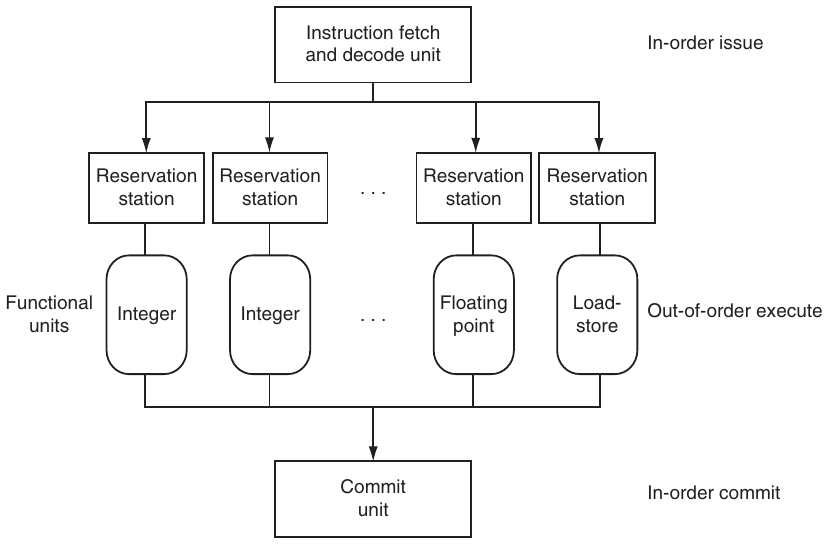
\includegraphics[width=\textwidth]{./figures/dynamically_scheduled_pipeline.png}
                        \begin{itemize}
                          \item The \alert{first unit} fetches instructions, decodes them, and sends each instruction to a corresponding \alert{functional unit} for execution. Each functional unit has buffers, called \alert{reservation stations}. As soon as the buffer contains all its operands and the functional unit is ready to execute, the result is calculated. When the result is completed, it is sent to any \alert{reservation stations} waiting for this particular result as well as to the \alert{commit unit}
                          \item \alert{Commit unit:} The unit in a dynamic or out-of-order execution pipeline that decides when it is safe to release the result of an operation to programmervisible registers and memory
                          \item \alert{Reservation station:} A buffer within a functional unit that holds the operands and the operation
                          \item \alert{Reorder buffer:} The buffer in the commit unit that holds results in a dynamically scheduled processor until it is safe to store the results to memory or a register
                          \item \alert{Reasons for Dynamic Pipeline Scheduling:}
                            \begin{itemize}
                              \item not all stalls are predictable (cache misses in the memory hierarchy cause unpredictable stalls)
                              \item the processor speculates on branch outcomes using dynamic branch prediction, it cannot know the exact order of instructions at compile time
                              \item as the pipeline latency and issue width change from one implementation to another, the best way to compile a code sequence also changes. Old legacy code will get much of the benefit of a new implementation without the need for recompilation
                            \end{itemize}
                        \end{itemize}
                      \end{minipage}
                    }
                  }
                  child {
                    node {Out-of-order execution
                      \resizebox{\textwidth}{!}{
                        \begin{minipage}[t]{8cm}
                          \begin{itemize}
                            \item A situation in pipelined execution when an instruction blocked from executing does \alert{not} cause the \alert{following instructions} to \alert{wait}
                          \end{itemize}
                        \end{minipage}
                      }
                    }
                  }
                  child {
                    node {In-order commit
                      \resizebox{\textwidth}{!}{
                        \begin{minipage}[t]{8cm}
                          \begin{itemize}
                            \item A commit in which the results of pipelined execution are written to the programmer visible state in the \alert{same order} that instructions are fetched.
                            \item To make programs behave as if they were running on a simple in-order pipeline
                          \end{itemize}
                        \end{minipage}
                      }
                    }
                  }
                }
              }
            }
          }
          child {
            node {Stages
              \resizebox{\textwidth}{!}{
                \begin{minipage}[t]{10cm}
                  \begin{itemize}
                    \item \alert{IF (Instruction Fetch):} Fetch instruction from memory
                    \item \alert{ID (Instruction Decode):} Read from register file and decode the instruction
                    \item \alert{EX (Execution):} Execute the operation or calculate an address
                    \item \alert{MEM (Memory):} Access an operand in data memory (if necessary)
                    \item \alert{WB (Write Back):} Write the result into a register (if necessary)
                  \end{itemize}
                \end{minipage}
              }
            }
          }
          child {
            node {Hazards
              \resizebox{\textwidth}{!}{
                \begin{minipage}[t]{8cm}
                  \begin{itemize}
                    \item situation in pipelining when the next instruction cannot execute in the following clock cycle
                  \end{itemize}
                \end{minipage}
              }
            }
              child {
                node {Data Hazard
                  \resizebox{\textwidth}{!}{
                    \begin{minipage}[t]{8cm}
                      \begin{itemize}
                        \item When a planned instruction cannot execute in the proper clock cycle because data that are needed to execute the instruction are not yet available
                        \item Also called a \alert{pipeline data hazard}
                        % \item Need to wait for previous instruction to complete its data read/write
                      \end{itemize}
                    \end{minipage}
                  }
                }
                child {
                  node {Double Data Hazard
                    \resizebox{\textwidth}{!}{
                      \begin{minipage}[t]{8cm}
                        \begin{itemize}
                          \item Want to use the most recent hazard if two happen after another (e.g. \texttt{add x1,x1,x2}, \texttt{add x1,x1,x3}, \texttt{add x1,x1,x4})
                        \end{itemize}
                      \end{minipage}
                    }
                  }
                }
                child {
                  node {True data dependency / read-after-write (RAW) hazard}
                    child {
                      node (forwarding) { Forwarding
                        \resizebox{\textwidth}{!}{
                          \begin{minipage}[t]{8cm}
                            \begin{itemize}
                              \item A method of resolving a data hazard by retrieving the missing data element from internal buffers rather than waiting for it to arrive from programmervisible registers or memory
                              \item Also called \alert{bypassing}
                              \item \alert{Forwarding unit:} Controls the ALU multiplexors to replace the value from a general-purpose register with the value from the proper pipeline register
                              % \begin{itemize}
                              %   \item  chooses the pipeline register for a register input to the ALU
                              % \end{itemize}
                            \end{itemize}
                          \end{minipage}
                        }
                      }
                      child {
                        node {Data Hazards in ALU Instructions
                          \resizebox{\textwidth}{!}{
                            \begin{minipage}[t]{12cm}
                              \begin{itemize}
                                \item \alert{Data hazards when:}
                                \begin{itemize}
                                  \item Forward from \texttt{EX/MEM} pipeline registers:
                                  \begin{itemize}
                                    \item \texttt{EX/MEM.RegisterRd = ID/EX.RegisterRs1}
                                    \item \texttt{EX/MEM.RegisterRd = ID/EX.RegisterRs2}
                                  \end{itemize}
                                  \item Forward from \texttt{MEM/WB} pipeline registers:
                                  \begin{itemize}
                                    \item \texttt{MEM/WB.RegisterRd = ID/EX.RegisterRs1}
                                    \item \texttt{MEM/WB.RegisterRd = ID/EX.RegisterRs2}
                                  \end{itemize}
                                \end{itemize}
                              \end{itemize}
                              \centering
                              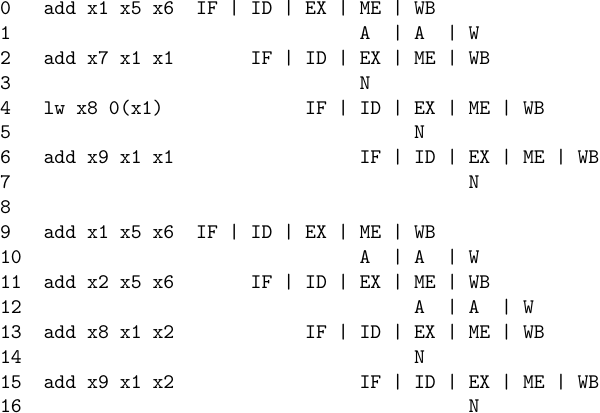
\includegraphics[width=\textwidth]{./figures/hazards_alu_instructions.png}
                              \begin{itemize}
                                \item \alert{First Chance \texttt{ME}:} $1$st instruction is in \texttt{EX}, $2$nd instruction is in \texttt{ID} and $3$rd instruction is in \texttt{IF}. A \texttt{NOP} is also an instruction:
                                \begin{itemize}
                                  \item forward from \texttt{EX/ME} to the corresponding stage if the \texttt{Need} of the $i$st instruction is in the \alert{corresponding} stage
                                  \item go to \alert{Second Chance} if the \texttt{Need} of the $i$st instruction is in a \alert{higher} or \alert{lower} stage
                                  \item no special action if there's \alert{no dependency}
                                \end{itemize}
                                \item \alert{Second Chance \texttt{WB}:} $1$st instruction is in \texttt{MEM}, $2$nd instruction is in \texttt{EX} and $3$rd instruction is in \texttt{ID}. A \texttt{NOP} is also an instruction:
                                \begin{itemize}
                                  \item forward from \texttt{ME/WB} to the corresponding stage if the \texttt{Need} of the $i$st instruction is in the \alert{corresponding} stage
                                  \item stall if the \texttt{Need} of the $i$st instruction is in a \alert{lower} stage
                                  \item no special action if the \texttt{Need} of the $i$st instruction is in a \alert{higher} stage as it will already be written to register when the instruction reaches it's higher stage with the \alert{Need}
                                \end{itemize}
                              \item this procedure just looks at the preceding stages of the \alert{single cycle diagram} (\alert{column} within the \alert{multicycle diagram} read from the \alert{bottom}) as \alert{forwarding} can only happen within the single cycle diagramm
                              \end{itemize}
                            \end{minipage}
                          }
                        }
                      }
                    }
                    child [level 7/.append style={level distance=5cm, sibling angle=40}] {
                      node {Pipeline stall
                        \resizebox{\textwidth}{!}{
                          \begin{minipage}[t]{8cm}
                            \begin{itemize}
                              \item A stall initiated in order to resolve a hazard
                              \item Also called bubble
                              \begin{itemize}
                                \item we can insert a \alert{bubble} into the pipeline by changing the EX, MEM, and WB control fields of the ID/EX \alert{pipeline register} to $0$. These benign control values are \alert{percolated forward at each clock cycle} with the proper effect: no registers or memories are written if the control values are all $0$
                              \end{itemize}
                              \item \alert{Nop:} An instruction that does no operation to change state
                              \begin{itemize}
                                \item \alert{nops} act like \alert{bubbles}
                              \end{itemize}
                              \item \alert{Hazard detection unit:} It operates during the ID stage so that it can insert the stall between the load and the instruction dependent on it
                              \begin{itemize}
                                \item The hazard detection unit controls the writing of the PC and IF/ID registers plus the multiplexor that chooses between the real control values and all 0s. The hazard detection unit stalls and deasserts the control fields if the load-use hazard test above is true
                              \end{itemize}
                              % \begin{itemize}
                              %    \item deasserting all seven control signals (setting them to $0$) in the EX, MEM, and WB stages will create a \enquote{do nothing} or nop instruction
                              % \end{itemize}
                            \end{itemize}
                          \end{minipage}
                        }
                      }
                        child {
                          node (datahazardsforbranches) {Data Hazards for Branches
                            \resizebox{\textwidth}{!}{
                              \begin{minipage}[t]{12cm}
                                \begin{itemize}
                                  \item If a comparison register is a destination of 2nd or 3rd preceding ALU instruction
                                  \begin{itemize}
                                    \item Can resolve using forwarding
                                  \end{itemize}
                                  \item If a comparison register is a destination of preceding ALU instruction or 2nd preceding load instruction
                                  \begin{itemize}
                                    \item Need $1$ stall cycle
                                  \end{itemize}
                                  \item  If a comparison register is a destination of immediately preceding load instruction
                                  \begin{itemize}
                                    \item Need $2$ stall cycles
                                  \end{itemize}
                                \end{itemize}
                                \centering
                                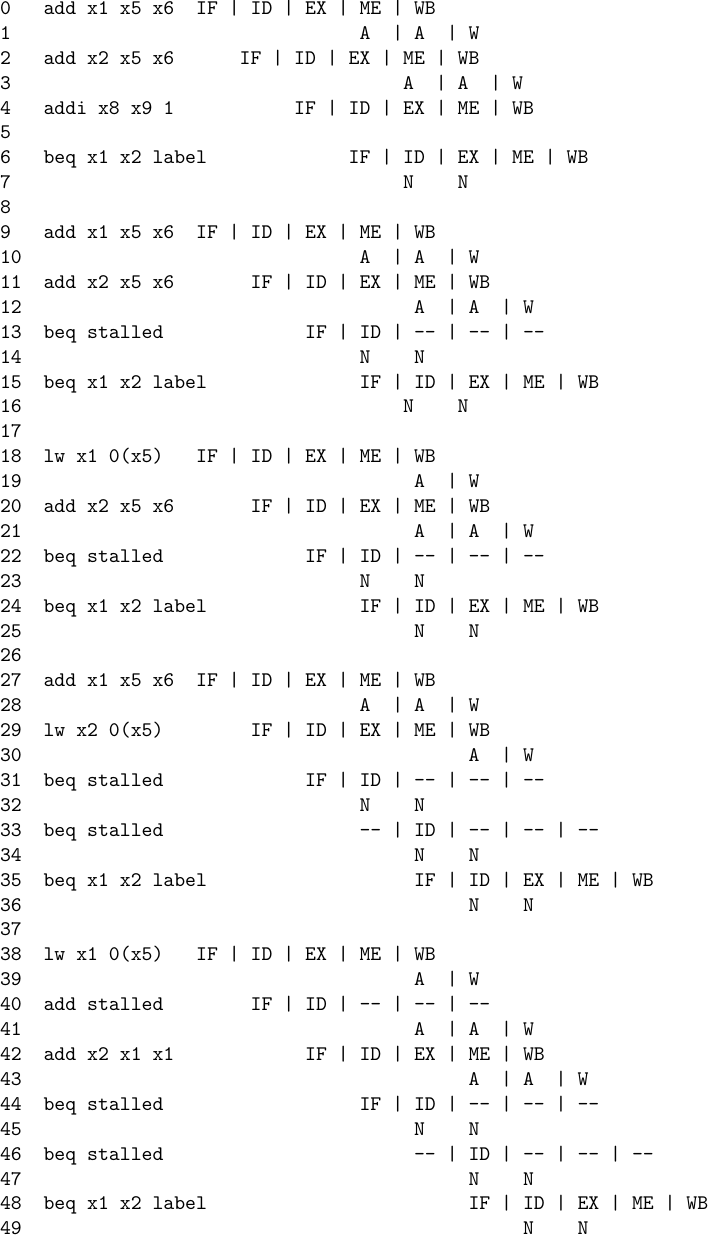
\includegraphics[width=\textwidth]{./figures/hazards_branches.png}
                              \end{minipage}
                            }
                          }
                        }
                        child {
                          node (loadusedatahazard) {Load-Use Data Hazard
                            \resizebox{\textwidth}{!}{
                              \begin{minipage}[t]{12cm}
                                \begin{itemize}
                                  \item A specific form of data hazard in which the data being loaded by a load instruction have not yet become available when they are needed by another instruction
                                  \item Load-use hazard when \texttt{ID/EX.MemRead and ((ID/EX.RegisterRd = IF/ID.RegisterRs1) or (ID/EX.RegisterRd = IF/ID.RegisterRs2))}
                                \end{itemize}
                                \centering
                                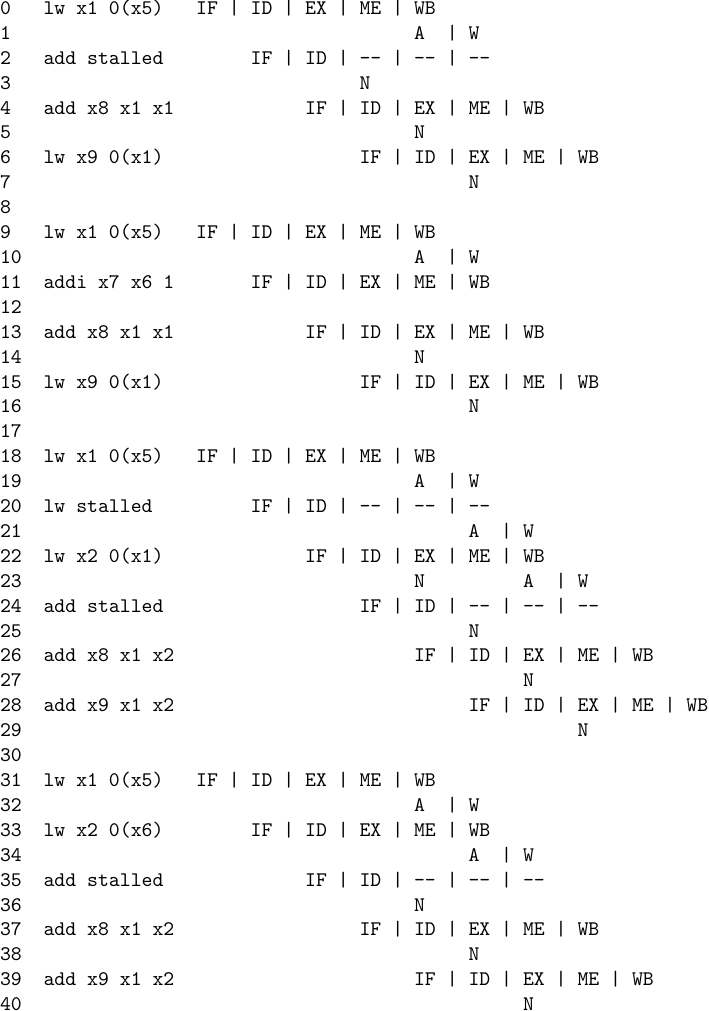
\includegraphics[width=\textwidth]{./figures/hazard_load_use.png}
                                \begin{itemize}
                                  \item \alert{Only chance \texttt{WB}:} $1$st instruction is in \texttt{MEM}, $2$nd instruction is in \texttt{EX} and $3$rd instruction is in \texttt{ID}. A \texttt{NOP} is also an instruction:
                                  \begin{itemize}
                                    \item forward from \texttt{MEM/WB} to the corresponding stage if the \texttt{Need} of the $i$st instruction is in the \alert{corresponding} stage
                                    \item stall if the \texttt{Need} of the $i$st instruction is in a \alert{lower} stage
                                    \item no special action if the \texttt{Need} of the $i$st instruction is in a \alert{higher} stage or there's \alert{no dependency}
                                  \end{itemize}
                                \end{itemize}
                                \begin{itemize}
                                  \item A $\overset{\wedge}{=}$ zum Beginn dieser Stage sind die Registerinhalte verfügbar
                                  \item W $\overset{\wedge}{=}$ die gewünschten Daten wurden bereits in die Registerfile geschrieben, kein Forwarding mehr nötig
                                  \item N $\overset{\wedge}{=}$ zum Beginn dieser Stage werden die Registerinhalte gebraucht
                                \end{itemize}
                              \end{minipage}
                            }
                          }
                        }
                    }
                }
                child {
                  node {Anti-dependence and Output dependence
                    \resizebox{\textwidth}{!}{
                      \begin{minipage}[t]{10cm}
                        \begin{itemize}
                          \item An \alert{Antidependence} between instructions i and j occurs when instruction j
writes a register or memory location that instruction i reads. The original
ordering must be preserved to ensure that i reads the correct value.  An antidependence can lead to a \alert{write-after-read (WAR) hazard}.
                          \item An \alert{Output dependence} occurs when instructions i and j write the same
register or memory location. The ordering between the instructions must be
preserved to ensure that the value finally written corresponds to instruction j. An output dependence can lead to a \alert{write-after-write (WAW) hazard}.
                        \end{itemize}
                      \end{minipage}
                    }
                  }
                }
              }
              child {
                node {Control Hazard
                  \resizebox{\textwidth}{!}{
                    \begin{minipage}[t]{8cm}
                      \begin{itemize}
                          \item When the proper instruction cannot execute in the proper pipeline clock cycle because the instruction that was fetched is not the one that is needed; that is, the flow of instruction addresses is not what the pipeline expected
                          \item Also called branch hazard
                        % \item Deciding on control action depends on previous instruction
                      \end{itemize}
                    \end{minipage}
                  }
                }
                  child {
                    node {Stall on Branch
                      \resizebox{\textwidth}{!}{
                        \begin{minipage}[t]{8cm}
                          \begin{itemize}
                            \item Wait until branch outcome determined before fetching next instruction
                          \end{itemize}
                        \end{minipage}
                      }
                    }
                  }
                  child {
                    node {Branch Prediction
                      \resizebox{\textwidth}{!}{
                        \begin{minipage}[t]{8cm}
                          \begin{itemize}
                            \item A method of resolving a branch hazard that assumes a given outcome for the conditional branch and proceeds from that assumption rather than waiting to ascertain the actual outcome
                          \end{itemize}
                        \end{minipage}
                      }
                    }
                      child {
                        node {Static branch prediction
                          \resizebox{\textwidth}{!}{
                            \begin{minipage}[t]{8cm}
                              \begin{itemize}
                                \item Based on \alert{typical branch behavior}
                                \item \alert{Example:} Loop branches $\rightarrow$ Predict backward branches taken, Predict forward branches not taken
                              \end{itemize}
                            \end{minipage}
                          }
                        }
                      }
                      child {
                        node {Dynamic branch prediction
                          \resizebox{\textwidth}{!}{
                            \begin{minipage}[t]{8cm}
                              \begin{itemize}
                                \item Prediction of branches at runtime using runtime information
                              \end{itemize}
                            \end{minipage}
                          }
                        }
                          child {
                            node (1bitpredictor) {1-Bit Predictor
                              \resizebox{\textwidth}{!}{
                                \begin{minipage}[t]{8cm}
                                  \begin{itemize}
                                    \item \alert{Inner loop branches mispredicted twice:}
                                    \begin{itemize}
                                      \item Mispredict as \alert{taken} on last iteration of inner loop
                                      \item Then mispredict as \alert{not taken} on first iteration of inner loop next time around
                                    \end{itemize}
                                  \end{itemize}
                                \end{minipage}
                              }
                            }
                              child {
                                node (branchpredictionbuffer) {Branch Prediction Buffer
                                  \resizebox{\textwidth}{!}{
                                    \begin{minipage}[t]{8cm}
                                      \begin{itemize}
                                        \item A small memory that is \alert{indexed by the lower portion of the address of the branch instruction} and that contains one or more bits indicating whether the \alert{branch was recently taken or not}
                                        \item  If the hint turns out to be wrong, the incorrectly predicted instructions are \alert{deleted}, the prediction bit is \alert{inverted} and \alert{stored back}, and the proper sequence is fetched and executed
                                        \item Also called \alert{branch history table}
                                        \item we don’t know, in fact, if the prediction is the right one, it may have been put there by another conditional branch that has the \alert{same low-order address bits}. However, this \alert{doesn’t affect correctness}
                                      \end{itemize}
                                    \end{minipage}
                                  }
                                }
                              }
                          }
                          child {
                            node (2bitpredictor) {2-Bit Predictor
                              \resizebox{\textwidth}{!}{
                                \begin{minipage}[t]{8cm}
                                  \begin{itemize}
                                    \item a \alert{prediction must be wrong twice} before it is changed
                                  \end{itemize}
                                  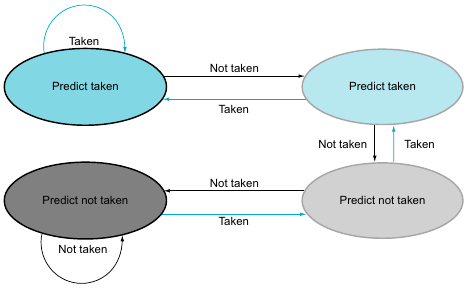
\includegraphics[width=\textwidth]{./figures/2_bit_predictor.png}
                                \end{minipage}
                              }
                            }
                          }
                          child {
                            node {Branch target buffer
                              \resizebox{\textwidth}{!}{
                                \begin{minipage}[t]{8cm}
                                  \begin{itemize}
                                    \item A structure that caches the destination PC or destination instruction for a branch. It is usually organized as a cache with tags, making it more costly than a simple prediction buffer
                                    \item A branch predictor tells us whether a conditional branch is taken, but still requires the calculation of the branch target
                                    \begin{itemize}
                                      \item In the five-stage pipeline, this calculation takes one cycle, meaning that taken branches will have a \alert{one-cycle penalty}. One approach is to use a cache to hold the destination program counter or destination instruction using a \alert{branch target buffer}
                                    \end{itemize}
                                  \end{itemize}
                                \end{minipage}
                              }
                            }
                          }
                      }
                      child {
                        node {Flush Instructions
                          \resizebox{\textwidth}{!}{
                            \begin{minipage}[t]{8cm}
                              \begin{itemize}
                                \item To discard instructions in a pipeline, usually due to an unexpected event
                              \end{itemize}
                              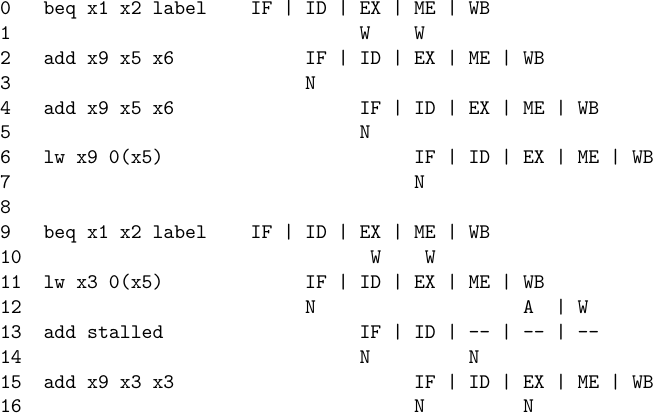
\includegraphics[width=\textwidth]{./figures/hazards_control_branch.png}
                              \begin{itemize}
                                \item The calculated adddress can't immediately be transmitted from the ID-Stage to the IF-Stage, because the IF-Stage already has a new instruction loaded. So only when the branch instruction reaches it's MEM-Stage, the instruction at the calculated address can be loaded in the IF-Stage
                              \end{itemize}
                            \end{minipage}
                          }
                        }
                      }
                  }
              }
              child {
                node {Structural Hazard
                  \resizebox{\textwidth}{!}{
                    \begin{minipage}[t]{8cm}
                      \begin{itemize}
                        \item When a planned instruction cannot execute in the proper clock cycle (Pipelining: Stage) because the hardware does not support the combination of instructions that are set to execute
                        \item Separate instruction / data caches
                        \begin{itemize}
                          \item Modified Harvard Architecture (Competition delayed to next higher level 2 and level 3 cache) and not Van-Neumann Architecture
Same component several times (enough ALU's)
                        \end{itemize}
                        % \item A required resource is busy
                      \end{itemize}
                    \end{minipage}
                  }
                }
                  % child {
                  %   node {Data Race
                  %     \resizebox{\textwidth}{!}{
                  %       \begin{minipage}[t]{8cm}
                  %         \begin{itemize}
                  %           \item Two memory accesses form a data race if they are from different threads to the same location, at least one is a write, and they occur one after another.
                  %         \end{itemize}
                  %       \end{minipage}
                  %     }
                  %   }
                  % }
              }
          }
        }
        child {
          node (multicycle) {Multicycle
            \resizebox{\textwidth}{!}{
              \begin{minipage}[t]{8cm}
                \begin{itemize}
                  \item In a multicycle implementation, each step in the execution will take 1 clock cycle. The multicycle implementation allows a functional unit to be used more than once per instruction, as long as it is used on different clock cycles.
                  \item \alert{$\#clock\ cycles$ for each instruction class:}
                  \begin{itemize}
                    \item \alert{Loads:} $5$
                    \item \alert{Stores:} $4$
                    \item \alert{ALU instructions:} $4$
                    \item \alert{Branches:} $3$
                  \end{itemize}
                \end{itemize}
              \end{minipage}
            }
          }
        }
    }
    child [level 2/.append style={sibling angle=50}] {
      % https://stackoverflow.com/questions/52611434/tikz-mindmaps-overriding-level-distance-and-sibling-angle-for-a-specific-node
      node {Exploiting Memory Hierarchy
        \resizebox{\textwidth}{!}{
          \begin{minipage}[t]{8cm}
            \begin{itemize}
              \item \alert{Temporal locality:} The locality principle stating that if a data location is referenced then it will tend to be referenced again soon.
              \item \alert{Spatial locality:} The locality principle stating that if a data location is referenced, data locations with nearby addresses will tend to be referenced soon.
              \item \alert{Static random access:} memory (SRAM) Also memory built as an integrated circuit, but faster and less dense than DRAM.
            \end{itemize}
          \end{minipage}
        }
      }
      child {
        node {Dependability
          \resizebox{\textwidth}{!}{
            \begin{minipage}[t]{10cm}
              \begin{itemize}
                \item \alert{Dependability Measures:}
                \begin{itemize}
                  \item \alert{Mean time between failures:} $MTBF = MTTF + MTTR$
                  \item \alert{Availability:} $\displaystyle \frac{MTTF}{MTTF + MTTR}$
                  \begin{itemize}
                    \item \alert{mean time to repair:} $MTTR$
                    \item \alert{mean time to failure:} $MTTF$
                  \end{itemize}
                \item three ways to improve MTTF:
                \begin{enumerate}
                  \item \alert{Fault avoidance:} Preventing fault occurrence by construction.
                  \item \alert{Fault tolerance:} Using redundancy to allow the service to comply with the service specification despite faults occurring.
                  \item \alert{Fault forecasting:} Predicting the presence and creation of faults, allowing the component to be replaced before it fails.
                \end{enumerate}
                \end{itemize}
              \end{itemize}
            \end{minipage}
          }
        }
          child {
            node {Hamming Error Correction Code (ECC)
              \resizebox{\textwidth}{!}{
                \begin{minipage}[t]{10cm}
                  \begin{itemize}
                    \item fault tolerance
                    \item $N = n + k$
                    \begin{itemize}
                      \item $N \overset{\wedge}{=} \#bits\_of\_codeword$
                      \item $n \overset{\wedge}{=} \#bits\_of\_dataword$
                      \item $k \overset{\wedge}{=} \#parity\_bits$
                    \end{itemize}
                    \item $N = 2^k - 1$, $k = log_{2}(N + 1)$ (for SEC)
                    \item $N = 2^{k-1}$, $k = log_{2}(N) + 1$ (for SECDED)
                    \item $n \le N - k = 2^k - k - 1$ (for SEC)
                    \item $n \le N - k = 2^{k-1} - k$ (for SECDED)
                    \item \alert{Notation:} $(N, n)$-Code
                    \item an den Bitpositionen im Codewort kommen nur Datenbits vor
                  \end{itemize}
                \end{minipage}
              }
            }
              child {
                node {Single-Error Correcting (SEC)
                  \resizebox{\textwidth}{!}{
                    \begin{minipage}[t]{12cm}
                      \begin{itemize}
                        \item Hamming Distance $3$
                        \item einen oder zwei Bitfehler in einem Datenblock erkennen
                        \item einen Bitfehler korrigieren
                        \item Bei zwei Bitfehlern liefert der Decoder ein gültiges, aber falsches Codewort
                        % \item Hamming Weight $3$
                        % \item provides single error correction, 2 bit error detection
                      \end{itemize}
                    \end{minipage}
                  }
                }
              }
              child {
                node {Single-Error Correcting and Double-Error-Detecting (SECDED)
                  \resizebox{\textwidth}{!}{
                    \begin{minipage}[t]{14cm}
                      \begin{itemize}
                        \item ein weiteres Paritätsbit angefügt, in das alle binären Stellen des nicht erweiterten Hamming-Code einfließen
                        \item nur sinnvoll, wenn das Codegewicht ungerade ist, da nur dann zusätzliche Information in diesem zusätzlichen Kontrollbit vorhanden ist.
                        \item Hamming Distance $4$
                        \item bis zu drei Bitfehler in einem Datenblock erkennen
                        \item einen Bitfehler korrigieren
                        \item zwei Bitfehler werden bei dem erweiterten Hamming-Code als fehlerhaftes (ungültiges) Codewort erkannt, welches nicht korrigierbar ist
                        % \item \alert{Decoding:} Let $H = SEC$ parity bits (Syndrome vector, the bit index the parity bits are pointing at), $p_n$ even if the transmitted and the determined additional parity bit match:
                        % \begin{itemize}
                        %   \item $H=0$ (even), $p_n$ even (match), no error
                        %   \item $H\ne 0$ (odd), $p_n$ odd (don't match), correctable single bit error
                        %   \item $H=0$ (even), $p_n$ odd (don't match), error in $p_n$ bit
                        %   \item $H\ne 0$ (odd), $p_n$ even (match), double error occurred
                        \item \alert{Decoding:} $H \overset{\wedge}{=}$ where the SEC-parity bits are pointing at,
                          $p_{n,t} \overset{\wedge}{=}$ transmitted DED-parity bit, $p_{n,d} \overset{\wedge}{=}$ determined DED-parity bit (DED-parity can also be called extra bit)
                        \begin{itemize}
                          \item $H=0$ (or SEC-parity bits detected no error), $p_{n,t} = p_{n,d}$ (or if all bits together are even, xor $0$) $\Rightarrow$ no error
                          \item $H\ne 0$ (or SEC-parity bits detected error), $p_{n,t} \ne p_{n,d}$ (or if all bits together are odd, xor $1$) $\Rightarrow$ correctable single bit error
                          \item $H=0$ (or SEC-parity bits detected no error), $p_{n,t} \ne p_{n,d}$ (or if all bits together are odd, xor $1$) $\Rightarrow$ error in $p_n$ bit
                          \item $H\ne 0$ (or SEC-parity bits detected error), $p_{n,t} = p_{n,d}$ (or if all bits together are even, xor $0$) $\Rightarrow$ double error occurred
                        \end{itemize}
                      \end{itemize}
                    \end{minipage}
                  }
                }
              }
              child {
                node {Hamming weight
                  \resizebox{\textwidth}{!}{
                    \begin{minipage}[t]{8cm}
                      \begin{itemize}
                        \item number of symbols that are different from the zero-symbol of the alphabet used
                        \item it is equivalent to the Hamming distance from the all-zero string of the same length
                      \end{itemize}
                      \centering
                      $\begin{tabular}{|l|l|}
                      \hline \multicolumn{1}{|c|}{ String } & Hamming weight \\
                      \hline 11101 & 4 \\
                      \hline 11101000 & 4 \\
                      \hline 00000000 & 0 \\
                      \hline
                      \end{tabular}$
                    \end{minipage}
                  }
                }
              }
              child {
                node {Hamming Distance
                  \resizebox{\textwidth}{!}{
                    \begin{minipage}[t]{14cm}
                      \begin{itemize}
                        \item Bei Codes mit Hamming-Abstand h können alle $d = h-1$-Bit-Fehler erkannt werden
                        % und alle $u = h-2$-Bit Fehler erkannt aber nicht korrigiert werden.
                        \item Bei Codes mit Hamming-Abstand h können alle $c = \lfloor\frac{h-1}{2}\rfloor$-Bit-Fehler korrigiert werden werden
                        \item Bei $h \,{=}\, 2$ können alle 1-Bit-Fehler erkannt werden. Um die Fehler auch korrigieren zu können, muss die Hamming-Distanz auf mindestens $h = 2c+1$ vergrößert werden
                        \begin{itemize}
                          \item \alert{error detection code (EDC):} A code that enables the detection of an error in data, but not the precise location and, hence, correction of the error
                        \end{itemize}
                        \item Bei $h \,{=}\, 3$ können alle 1-Bit-Fehler erkannt und korrigiert werden. Treten 2-Bit-Fehler auf, werden diese unter Umständen falsch \enquote{korrigiert}, da das fehlerhafte Wort möglicherweise den Abstand 1 zu einem anderen gültigen Codewort hat
                        \item Bei $h \,{=}\, 4$ können alle 1-Bit-Fehler erkannt und korrigiert werden. Treten 2-Bit-Fehler auf, können diese zwar erkannt, aber nicht mehr korrigiert werden
                        \item Der Hamming-Abstand eines Codes ist notwendigerweise eine positive natürliche Zahl. Ein Code mit Hamming-Abstand 0 ist nicht möglich, da sich in diesem Fall zwei Codewörter nicht unterscheiden ließen.
                      \end{itemize}
                    \end{minipage}
                  }
                }
                  child {
                    node {of two Codewords
                      \resizebox{\textwidth}{!}{
                        \begin{minipage}[t]{8cm}
                          \begin{itemize}
                            \item number of positions at which corresponding symbols are different
                          \end{itemize}
                        \end{minipage}
                      }
                    }
                  }
                  child {
                    node {of two Codes
                      \resizebox{\textwidth}{!}{
                        \begin{minipage}[t]{8cm}
                          \begin{itemize}
                            \item minimum of all distances between codewords within the code
                          \end{itemize}
                        \end{minipage}
                      }
                    }
                  }
              }
          }
      }
      child {
        node {Paging
          \resizebox{\textwidth}{!}{
            \begin{minipage}[t]{14cm}
              \begin{itemize}
                \item \alert{physical address:} An address in main memory
                \item \alert{virtual address:} An address that corresponds to a location in virtual space and is translated by address mapping to a physical address when memory is accessed
                \item \alert{address translation / mapping:} The process by which a virtual address is mapped to an address used to access memory
                \item A virtual memory block is called a \alert{page}, and a virtual memory miss is called a \alert{page fault}
                \begin{itemize}
                  \item \alert{Library analogy:} We can think of a virtual address as the title of a book and a physical address as the location of that book in the library, such as might be given by the Library of Congress call number
                \end{itemize}
                \item \alert{page fault:} An event that occurs when an accessed page is not present in main memory
                \item The number of bits in the \alert{page offset} field determines the \alert{page size}
                \item The number of pages addressable with the \alert{virtual address} can be different than the number of pages addressable with the \alert{physical address}
                \begin{itemize}
                  \item Having a larger number of \alert{virtual pages} than \alert{physical pages} is the basis for the illusion of larger amount of virtual memory
                \end{itemize}
                \item \alert{Write-through} will \alert{not} work for virtual memory, since writes take too long. Instead, virtual memory systems use \alert{write-back}.
                \item Many design choices in virtual memory systems are motivated by the \alert{high cost} of a \alert{page fault}
                \begin{itemize}
                  \item Page faults can be \alert{handled in software} because the overhead will be small compared to the disk access time. Software can afford to use clever algorithms for choosing how to place pages
                \end{itemize}
              \end{itemize}
              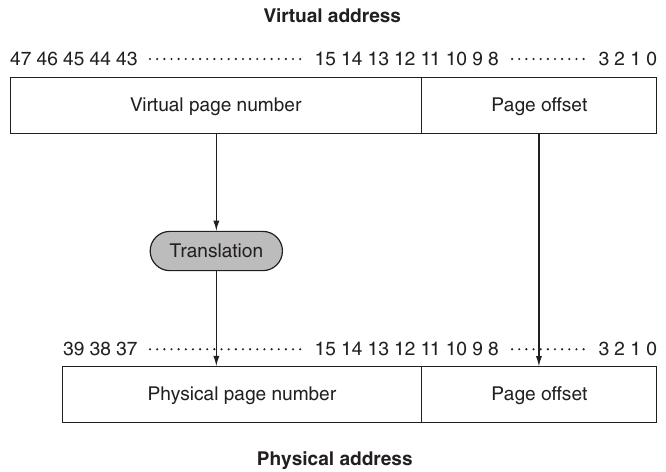
\includegraphics[width=\textwidth]{./figures/mapping_physical_to_virtual_address.png}
            \end{minipage}
          }
        }
        child {
          node {Page Table
            \resizebox{\textwidth}{!}{
              \begin{minipage}[t]{14cm}
                \begin{itemize}
                  \item \alert{Page table:} The table containing the virtual to physical address translations in a virtual memory system. The table, which is stored in memory, is typically indexed by the virtual page number; each entry in the table contains the physical page number for that virtual page if the page is currently in memory.
                  \item \alert{difficult} using \alert{fully associative} placement in locating an entry. Therefore in virtual memory systems one locates pages by using a \alert{page table}
                  \item A page table is \alert{indexed} by the \alert{page number} from the \alert{virtual address} to discover the corresponding \alert{physical page number}
                  \item Resides in \alert{main memory}. \alert{Each program} has its \alert{own page table}, which maps the virtual address space of that program to main memory
                  \item \alert{Library analogy:}, the page table corresponds to a mapping between \alert{book titles} and \alert{library locations}. Just as the card catalog may contain entries for books in \alert{another library} on campus rather than the local branch library, we will see that the page table may contain \alert{entries for pages not present in memory}
                  \item To \alert{indicate the location of the page table in memory}, the hardware includes a \alert{register} that points to the \alert{start of the page table}; we call this the \alert{page table register}
                  \item A \alert{valid bit} is used in each page table entry % , just as it was done in the cache
                  \begin{itemize}
                    \item If the bit is \alert{off}, the page is not present in main memory and a \alert{page fault} occurs
                    \item If the bit is \alert{on}, the page is \alert{in memory} and the entry contains the \alert{physical page number}
                  \end{itemize}
                  \item Because the \alert{page table contains} a mapping for \alert{every possible virtual page}, \alert{no tags} are \alert{required}
                  \item In \alert{cache terminology}, the \alert{index} that is used to access the page table consists of the \alert{full block address}, which in this case is the \alert{virtual page number}
                  \item if an \alert{page fault} occurs, the \alert{operating system must be given control}. This transfer is done with a \alert{exception mechanism}
                \end{itemize}
                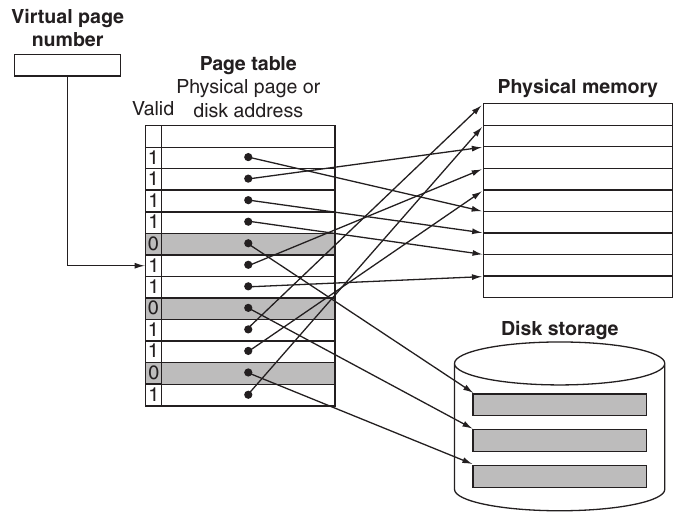
\includegraphics[width=\textwidth]{./figures/page_table.png}
              \end{minipage}
            }
          }
            child {
              node {Translation-lookaside buffer (TLB)
                \resizebox{\textwidth}{!}{
                  \begin{minipage}[t]{14cm}
                    \begin{itemize}
                      \item A \alert{cache} that keeps track of \alert{recently used address mappings} to try to \alert{avoid} an \alert{access to the page table}
                      \item Page tables are stored in main memory, every memory access by a program can take at least \alert{twice as long}: one memory access to obtain the physical address and a second access to get the data
                      \begin{itemize}
                        \item Key to improving access performance is to rely on \alert{locality of reference to the page table}
                        \item When a translation for a virtual page number is used, it will probably be needed again soon, because the references to the words on that page have both \alert{temporal} and \alert{spatial locality}
                      \end{itemize}
                      \item Each \alert{tag entry} in the TLB holds a \alert{portion of the virtual page number} and each \alert{data entry} of the TLB holds a \alert{physical page number}
                      \item Access the TLB \alert{instead} of the \alert{page table} on every reference, the TLB will need to include other \alert{status bits}
                      \item TLBs work fine with \alert{multi-level page tables} as well. The TLB simply loads the \alert{physical address} and \alert{protection tags} from the \alert{last level page table}
                      \item On every reference, we look up the virtual page number in the TLB:
                      \begin{itemize}
                        \item If we get a \alert{hit}, the physical page number is used to form the address, and the corresponding reference bit is turned on
                        \begin{itemize}
                          \item If the processor is performing a write, the dirty bit is also turned on
                        \end{itemize}
                        \item If a \alert{miss} in the TLB occurs, we must determine whether it is a page fault or merely a TLB miss
                        \begin{itemize}
                          \item If the \alert{page exists} in memory, then the TLB miss indicates only that the \alert{translation is missing}. In such cases, the processor can handle the TLB miss by loading the translation from the (last-level) page table into the TLB and then trying the reference again
                          \item If the \alert{page is not present} in memory, then the TLB miss indicates a \alert{true page fault}. In this case, the processor invokes the operating system using an exception
                        \end{itemize}
                      \end{itemize}
                      \item TLB misses can be handled either in \alert{hardware} or in \alert{software}. In practice, with care there can be little performance difference between the two approaches, because the basic operations are the same in either case
                      \item Because the TLB has many fewer entries than the number of pages in main memory, TLB misses will be much more frequent than true page faults
                      \item It would be more accurate to call it a \alert{translation cache}
                      \item \alert{Analogy:} TLB corresponds to that little \alert{piece of paper} we typically use to record the \alert{location of a set of books} we look up in the card catalog; rather than continually searching the \alert{entire catalog}, we record the location of several books and use the \alert{scrap of paper} as a cache of Library of Congress call numbers
                      \item can be implemented as small, fully associative TLBs or large TLBs with small associativity
                    \end{itemize}
                    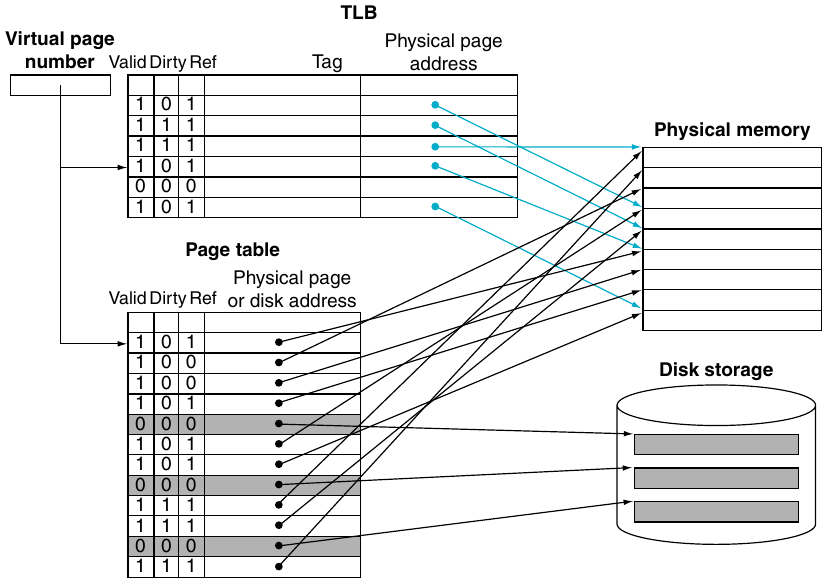
\includegraphics[width=\textwidth]{./figures/tlb.png}
                  \end{minipage}
                }
              }
              child {
                node {Replacement Scheme
                  \resizebox{\textwidth}{!}{
                    \begin{minipage}[t]{12cm}
                      \begin{itemize}
                        \item choosing the entry to replace becomes tricky since implementing a hardware \alert{LRU} scheme is \alert{too expensive}
                        \begin{itemize}
                          \item since TLB misses are \alert{much more frequent} than \alert{page faults} and thus must be handled more cheaply, one \alert{cannot afford} an expensive \alert{software algorithm}, as one can for page faults
                          \item As a result, many systems provide some support for \alert{randomly choosing an entry} to replace
                        \end{itemize}
                      \end{itemize}
                    \end{minipage}
                  }
                }
              }
              child {
                node {Write-back
                  \resizebox{\textwidth}{!}{
                    \begin{minipage}[t]{8cm}
                      \begin{itemize}
                        \item After a \alert{TLB miss occurs} and the missing translation has been retrieved from the page table, we will need to select a TLB entry to \alert{replace}
                        \begin{itemize}
                          \item Because the \alert{reference} and \alert{dirty bits} are \alert{contained in the TLB entry}, we need to \alert{copy} these bits \alert{back} to the \alert{page table entry} when we \alert{replace} an entry. These \alert{bits} are the only portion of the TLB entry that can be \alert{changed}
                        \end{itemize}
                        \item Some systems use other techniques to approximate the reference and dirty bits, eliminating the need to write into the TLB except to load a new table entry on a miss
                        \item is very efficient, since we expect the TLB miss rate to be still quite small
                        \item There can be an extra complication for \alert{write requests:} namely, the \alert{write access bit} in the TLB must be checked. This bit \alert{prevents} the program from \alert{writing into pages} for which it has \alert{only read access}. If the program attempts a write and the write access bit is \alert{off}, an \alert{exception} is generated
                      \end{itemize}
                    \end{minipage}
                  }
                }
              }
            }
        }
        child {
          node {Write Policy
            \resizebox{\textwidth}{!}{
              \begin{minipage}[t]{8cm}
                \begin{itemize}
                  \item Writes to the next level of the hierarchy (disk) can take millions of processor clock cycles; therefore, building a \alert{write buffer} to allow the system to \alert{write-through} to disk would be completely \alert{impractical}
                \end{itemize}
              \end{minipage}
            }
          }
            child {
              node {Write-back
                \resizebox{\textwidth}{!}{
                  \begin{minipage}[t]{10cm}
                    \begin{itemize}
                      \item Performing the \alert{individual writes} into the \alert{page in memory}, and \alert{copying} the page back to \alert{secondary memory} when it is \alert{replaced} in the main memory
                      \item \alert{advantage:}
                      \begin{itemize}
                        \item Because the disk \alert{transfer time} is small compared with its \alert{access time}, copying back an \alert{entire page} is much more efficient than writing \alert{individual words} back to the disk
                      \end{itemize}
                      \item \alert{dirty bit:} needed to track whether a page has been written since it was read into the memory, so one knows whether a page needs to be copied back when the operating system chooses to replace it
                      \begin{itemize}
                        \item The \alert{dirty bit} is set when \alert{any word} in a page is written
                        \item A modified page is often called a \alert{dirty page}
                      \end{itemize}
                    \end{itemize}
                  \end{minipage}
                }
              }
            }
        }
        child {
          node {Replacement schemes
            \resizebox{\textwidth}{!}{
              \begin{minipage}[t]{8cm}
                \begin{itemize}
                  \item When a page fault occurs, if \alert{all} the \alert{pages} in main memory are \alert{in use}, the operating system must choose a \alert{page} to \alert{replace}
                \end{itemize}
              \end{minipage}
            }
          }
            child {
              node {Least recently used (LRU)
                \resizebox{\textwidth}{!}{
                  \begin{minipage}[t]{12cm}
                    \begin{itemize}
                      \item Because we want to \alert{minimize} the number of \alert{page faults}, most operating systems try to choose a page that they hypothesize will not be needed soon. Using the \alert{past to predict the future}, operating systems follow the least recently used (LRU) replacement scheme
                      \item The operating system searches for the least recently used page, assuming that a page that has not been used in a long time is \alert{less likely to be needed} than a more \alert{recently accessed page}
                      \item \alert{reference / use / access bit} A field that is set whenever a page is accessed and that is used to implement LRU or other replacement schemes
                      \begin{itemize}
                        \item most operating systems \alert{approximate LRU} by keeping track of which pages have and which pages have not been recently used
                        \item operating system \alert{periodically} clears the reference bits and later records them so it can determine which pages were touched during a particular time period
                        \item With this \alert{usage information}, the operating system can select a page that is among the least recently referenced (detected by having its reference bit off)
                      \end{itemize}
                    \end{itemize}
                    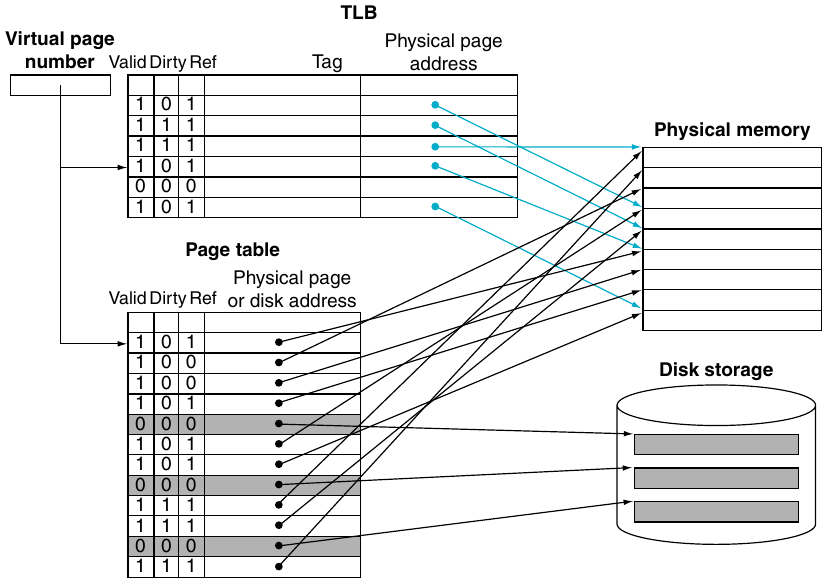
\includegraphics[width=\textwidth]{./figures/tlb.png}
                  \end{minipage}
                }
              }
            }
        }
        child {
          node {Virtual Memory
            \resizebox{\textwidth}{!}{
              \begin{minipage}[t]{12cm}
                \begin{itemize}
                  \item A technique that uses main memory as a \enquote{cache} for secondary storage
                  \item Main memory need contain only the active portions of the many virtual machines, just as a cache contains only the active portion of one program
                  \item \alert{Two major motivations for virtual memory:}
                  \begin{itemize}
                    \item To allow efficient and safe sharing of memory among several programs, such as for the memory needed by multiple virtual machines for Cloud computing
                    \item To remove the programming burdens of a small, limited amount of main memory
                  \end{itemize}
                  \item compile each program into its \alert{own address space}, a separate range of memory locations accessible only to this program.
                  \begin{itemize}
                    \item Virtual memory implements the \alert{translation} of a program’s address space to physical addresses
                    \item This translation process enforces \alert{protection} of a program’s address space from other virtual machines
                  \end{itemize}
                  \item \alert{protection:} A set of mechanisms for ensuring that multiple processes sharing the processor, memory, or I/O devices cannot interfere, intentionally or unintentionally, with one another by reading or writing each other’s data. These mechanisms also isolate the operating system from a user process.
                \end{itemize}
              \end{minipage}
            }
          }
            child {
              node {Swap Space
                \resizebox{\textwidth}{!}{
                  \begin{minipage}[t]{12cm}
                    \begin{itemize}
                      \item The space on the disk reserved for the full virtual memory space of a process
                      \item The virtual address alone does \alert{not} immediately tell us \alert{where the page is in secondary memory}.
                      \item \alert{Library analogy:} We \alert{cannot find the location} of a library book on the shelves just by \alert{knowing its title}. Instead, we \alert{go to the catalog} and \alert{look up the book}, obtaining an address for the location on the shelves, such as the Library of Congress call number
                      \item Because we do not know ahead of time when a page in memory will be replaced, the operating system usually creates the \alert{swap space} on flash memory or disk for all the pages of a process when it creates the process.
                      \begin{itemize}
                        \item it also creates a \alert{data structure} to record where each virtual page is stored on disk
                        \item This data structure may be part of the page table or may be an auxiliary data structure \alert{indexed in the same way} as the page table
                      \end{itemize}
                    \end{itemize}
                  \end{minipage}
                }
              }
            }
            child {
              node {Virtual Machine
                \resizebox{\textwidth}{!}{
                  \begin{minipage}[t]{10cm}
                    \begin{itemize}
                      \item broadest definition of VMs includes basically all emulation methods that provide a standard software interface, such as the Java VM
                      \item System virtual machines present the illusion that the users have an entire computer to themselves, including a copy of the operating system
                      \begin{itemize}
                        \item provide a complete system-level environment at the binary instruction set architecture (ISA) level
                      \end{itemize}
                      \item The software that supports VMs is called a virtual machine monitor (VMM) or hypervisor
                      \item VMM determines how to map virtual resources to physical resources
                      \item The underlying hardware platform is called the host, and its resources are shared among the guest VMs
                    \end{itemize}
                  \end{minipage}
                }
              }
            }
        }
      }
      child {
        node {Caching
          \resizebox{\textwidth}{!}{
            \begin{minipage}[t]{12cm}
              \begin{itemize}
                \item \alert{block (or line):} The minimum unit of information that can be either present or not present in a cache
                \item \alert{cache miss:} A request for data from the cache that cannot be filled because the data are not present in the cache
                \item \alert{miss / hit rate:} The fraction of memory accesses (not) found in a level of the memory hierarchy
                \item \alert{hit time:} The time required to access a level of the memory hierarchy, including the time needed to determine whether the access is a hit or a miss
                \item \alert{miss penalty:} The time required to fetch a block into a level of the memory hierarchy from the lower level, including the time to access the block, transmit it from one level to the other, insert it in the level that experienced the miss, and then pass the block to the requestor
                \begin{itemize}
                  \item \alert{two parts:} the latency to the first word and the transfer time for the rest of the block
                \end{itemize}
              \end{itemize}
            \end{minipage}
          }
        }
          child {
            node {Cache Performance
              \resizebox{\textwidth}{!}{
                \begin{minipage}[t]{10cm}
                  \begin{itemize}
                    \item $\text{D\_stall\_cycles} \begin{aligned}[t] & =\frac{\text { Memory\_accesses }}{\text { Program }} \times \text { Miss\_rate } \times \text { Miss\_penalty } \\
& =\frac{\text { Instructions} }{\text { Program }} \times \frac{\text { Misses }}{\text { Instruction }} \times \text { Miss\_penalty }
\end{aligned}
$
                    \item $\text{I\_stall\_cycles} \begin{aligned}[t] & = \text { Miss\_rate } \times \text { Miss\_penalty }
\end{aligned}
$
                    \item $Actual\_CPI = Base\_CPI + I\_stall\_cycles + D\_stall\_cycles$
                    \item Larger blocks exploit \alert{spatial locality} to \alert{lower miss rates}
                    \begin{itemize}
                      \item \alert{miss rate} may go up eventually if the block size becomes a \alert{significant fraction} of the \alert{cache size}, because the \alert{number of blocks} that can be held in the cache will become \alert{small}, and there will be a great deal of \alert{competition for those blocks}. As a result, a block will be bumped out of the cache before many of its words are accessed
                    \end{itemize}
                    \item Larger blocks increase the transfer time and hence the miss penalty
                  \end{itemize}
                \end{minipage}
              }
            }
              child {
                node {Multilevel cache
                  \resizebox{\textwidth}{!}{
                    \begin{minipage}[t]{12cm}
                      \begin{itemize}
                        \item A memory hierarchy with multiple levels of caches, rather than just a cache and main memory.
                        \item Close the gap further between the fast clock rates of modern processors and the increasingly long time required to access DRAMs
                        \begin{itemize}
                          \item Second-level cache accessed whenever a miss occurs in the primary cache
                          \item If the second-level cache contains the desired data, the miss penalty for the first-level cache will be essentially the access time of the second-level cache
                          \item If neither the primary nor the secondary cache contains the data, a main memory access is required, and a larger miss penalty is incurred
                        \end{itemize}
                        \item \alert{Miss penalty:} $\frac{T_{Main\_memory\_access}}{\frac{1}{f_{processor}}}$
                        \item with a two-level cache, total CPI is the sum of the stall cycles per instruction from both levels of cache and the base CPI:\\[0.25cm]
                          $\begin{aligned} Total\_CPI =\; &Base\_CPI + Miss\_rate\_to\_secondary\_cache \cdot Secondary\_cache\_miss\_penalty\\
                        &+ Miss\_rate\_to\_main\_memory \cdot Main\_memory\_miss\_penalty\end{aligned}$
                        \begin{itemize}
                          \item $Miss\_rate\_to\_secondary\_cache$ and $Miss\_rate\_to\_main\_memory$ are independant probabilities that there's an access to the corresponding second-level cache or main memory necessary % even though an access to main-memory can only happen if there was a miss in the second-level cache
                        \end{itemize}
                        \item \alert{usage:}
                        \begin{itemize}
                          \item a two-level cache structure allows the primary cache to focus on minimizing hit time to yield a shorter clock cycle or fewer pipeline stages, while allowing the secondary cache to focus on miss rate to reduce the penalty of long memory access times
                          \item With a larger total size, the secondary cache may use a larger block size than appropriate with a single-level cache. It often uses higher associativity than the primary cache given the focus of reducing miss rates
                        \end{itemize}
                      \end{itemize}
                    \end{minipage}
                  }
                }
              }
              child {
                node {Prefetching
                  \resizebox{\textwidth}{!}{
                    \begin{minipage}[t]{8cm}
                      \begin{itemize}
                        \item A technique in which \alert{data blocks} needed in the future are \alert{brought into the cache early} by using special instructions that specify the address of the block
                      \end{itemize}
                    \end{minipage}
                  }
                }
              }
              child {
                node {Memory Hierarchy
                  \resizebox{\textwidth}{!}{
                    \begin{minipage}[t]{8cm}
                      \begin{itemize}
                        \item A structure that uses multiple levels of memories; as the distance from the processor increases, the size of the memories and the access time both increase while the cost pert bit decreases
                      \end{itemize}
                    \end{minipage}
                  }
                }
              }
          }
          child {
            node {Write Policy
              \resizebox{\textwidth}{!}{
                \begin{minipage}[t]{8cm}
                  \begin{itemize}
                    \item \alert{steps instruction cache miss:}
                    \begin{enumerate}
                      \item Send the original PC value to the memory
                      \item Instruct main memory to perform a read and wait for the memory to complete its access
                      \item Write the cache entry, putting the data from memory in the data portion of the entry, writing the upper bits of the address (from the ALU) into the tag field, and turning the valid bit on if it was not on already
                      \item Restart the instruction execution at the first step, which will refetch the instruction, this time finding it in the cache
                    \end{enumerate}
                    \item control of the cache on a \alert{data access} is similiar: on a miss, we simply stall the processor until the memory responds with the data
                  \end{itemize}
                \end{minipage}
              }
            }
              child {
                node {Write-through
                  \resizebox{\textwidth}{!}{
                    \begin{minipage}[t]{8cm}
                      \begin{itemize}
                        \item \alert{write-through:} A scheme in which writes always update both the cache and the next lower level of the memory hierarchy, ensuring that data are always consistent between the two
                        \item would provide \alert{bad performance}. With a write-through scheme, every write causes the data to be written to main memory
                      \end{itemize}
                    \end{minipage}
                  }
                }
                child {
                  node {Write buffer
                    \resizebox{\textwidth}{!}{
                      \begin{minipage}[t]{12cm}
                        \begin{itemize}
                          \item solution to bad performance of \alert{write-through}
                          \item A queue that holds data while the data are waiting to be written to memory
                          \item After writing the data into the cache and into the write buffer, the processor can continue execution. When a write to main memory completes, the entry in the write buffer is freed
                          \item If the write buffer is full when the processor reaches a write, the processor must stall until there is an empty position in the write buffer
                          \begin{itemize}
                            \item If the rate at which the memory can complete writes is less than the rate at which the processor is generating writes, no amount of buffering can help, because writes are being generated faster than the memory system can accept them
                            \item The rate at which writes are generated may also be less than the rate at which the memory can accept them, and yet stalls may still occur. This can happen when the writes occur in bursts.
                          \end{itemize}
                        \end{itemize}
                      \end{minipage}
                    }
                  }
                }
              }
              child {
                node {Write-back
                  \resizebox{\textwidth}{!}{
                    \begin{minipage}[t]{8cm}
                      \begin{itemize}
                        \item \alert{write-back:} A scheme that handles writes by updating values only to the block in the cache, then writing the modified block to the lower level of the hierarchy when the block is replaced
                        \item \alert{dirty bit:} Means this \alert{cache line} was actually \alert{updated}. Only need to \alert{write back} if it's \alert{dirty} (if it was written)
                        \item delays writing and one can additionaly have a \alert{write buffer} again
                      \end{itemize}
                    \end{minipage}
                  }
                }
              }
          }
          child {
            node {Replacement schemes
              \resizebox{\textwidth}{!}{
                \begin{minipage}[t]{8cm}
                  \begin{itemize}
                    \item In an associative cache, we have a choice of which block to replace among the blocks in the selected set
                  \end{itemize}
                \end{minipage}
              }
            }
              child {
                node {Least recently used (LRU)
                  \resizebox{\textwidth}{!}{
                    \begin{minipage}[t]{10cm}
                      \begin{itemize}
                        \item \alert{least recently used (LRU):} A replacement scheme in which the block replaced is the one that has been unused for the longest time.
                        \item For a \alert{two-way set-associative cache}, tracking when the two elements were used can be implemented by keeping a single bit in each set and setting the bit to indicate an element whenever that element is referenced.
                        \begin{itemize}
                          \item As \alert{associativity increases}, implementing LRU gets \alert{harder}
                        \end{itemize}
                      \end{itemize}
                    \end{minipage}
                  }
                }
              }
              child {
                node {Pseudo-LRU
                  \resizebox{\textwidth}{!}{
                    \begin{minipage}[t]{8cm}
                      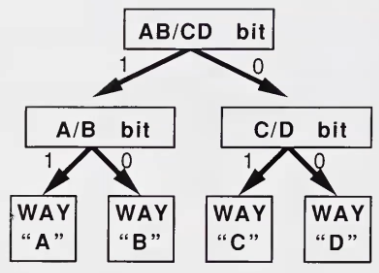
\includegraphics[width=\textwidth]{./figures/pseudo_lru.png}
                      \begin{itemize}
                        \item $A, B, C, A, B, C$, D is least recently used but:
                        \begin{itemize}
                          \item After the $C$ access the $AB/CD$-Bit would point to $AB$ and the $A/B$-Bit would point to A
                        \end{itemize}
                      \end{itemize}
                    \end{minipage}
                  }
                }
              }
              child {
                node {Random
                  \resizebox{\textwidth}{!}{
                    \begin{minipage}[t]{8cm}
                      \begin{itemize}
                        \item Candidate blocks are randomly selected, possibly using some hardware assistance.
                      \end{itemize}
                    \end{minipage}
                  }
                }
              }
          }
          child {
            node {Cache Coherence Protocols}
          }
          child {
            node {Types of Caches
              \resizebox{\textwidth}{!}{
                \begin{minipage}[t]{12cm}
                  \begin{itemize}
                    \item \alert{valid bit:} A field in the tables of a memory hierarchy that indicates that the associated block in the hierarchy contains valid data
                    \item \alert{tag:} A field in a table used for a memory hierarchy that contains the address information required to identify whether the associated block in the hierarchy corresponds to a requested word
                    \begin{itemize}
                      \item when determining a cache hit BlockOffset and Index of the address matches anyhow but to know if the other missing bits are also correct one also has to store the missing bits as Tag
                    \end{itemize}
                    \item \alert{index:} Used to select the block
                    \item \alert{cache miss:} A request for data from the cache that cannot be filled because the data are not present in the cache.
                    \item \alert{advantage} of increasing the degree of associativity is that it usually \alert{decreases the miss rate}
                    \item \alert{disadvantage} is a potential \alert{increase in the hit time}.
                    \begin{itemize}
                      \item \alert{costs} of an \alert{associative cache} are the \alert{extra comparators} and any \alert{delay} imposed by having to do the \alert{compare and select from among the elements of the set}
                    \end{itemize}
                  \end{itemize}
                  \centering
                  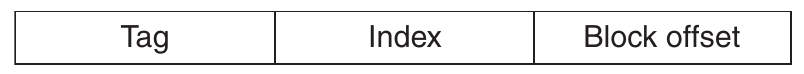
\includegraphics[width=0.5\textwidth]{./figures/three_portions_of_address.png}
                  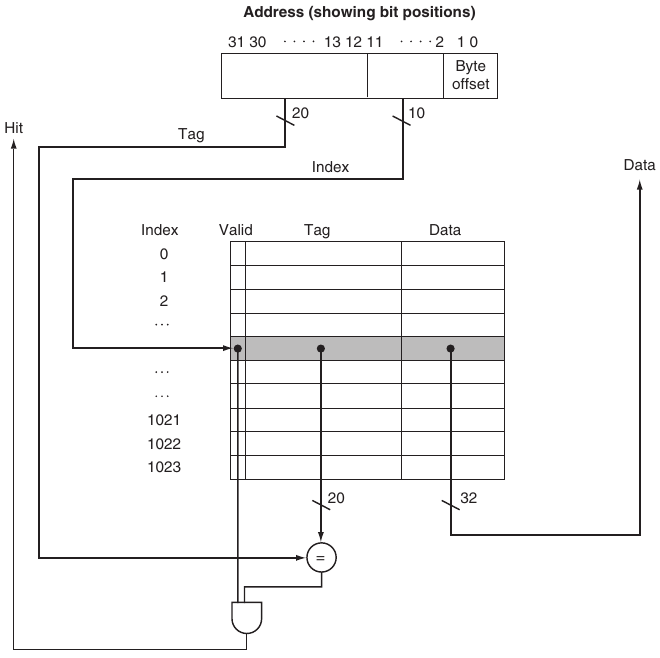
\includegraphics[width=0.5\textwidth]{./figures/direct_mapped.png}
                \end{minipage}
              }
            }
              child {
                node {Direct mapped (1-way associative)
                  \resizebox{\textwidth}{!}{
                    \begin{minipage}[t]{12cm}
                      \begin{itemize}
                        \item One choice for placement
                        \item is an \alert{one-way set-associative cache}
                        \item only a single comparator is needed, because the entry can be in only one block
                        \item $Block\ memory\ address = \lfloor \frac{Byte\ memory\ address}{Bytes\ per\ block}\rfloor$
                        \begin{itemize}
                          \item Block contains all addresses between\\[0.25cm]
                            $\displaystyle \left\lfloor\frac{\text { Byte address }}{\text { Bytes per block }}\right\rfloor \times Bytes\ per\ block$\\[0.25cm]and\\[0.25cm] $\displaystyle \left\lfloor\frac{\text { Byte address }}{\text { Bytes per block }}\right\rfloor \times \text { Bytes per block }+(\text { Bytes per block }-1)$
                        \end{itemize}
                        \item $\displaystyle Block\ cache\ address = (Block\ memory\ address)\ modulo\ (\#Blocks\ in\ cache)$
                        \item The \alert{cache size} is $2^n$ blocks, so $n$ bits are used for the index
                        \item The \alert{block size} is $2^m$ words ($2^{m+2}$ bytes, $2^{m+5}$ bits), so $m$ bits are used for the word within the block, and two bits are used for the byte part of the address
                        \item \alert{Size of the tag field:} $32 - (n + m + 2)$ (32-bit address)
                        \item $\displaystyle \#Blocks = \frac{Cache\ size}{Block\ size} = \frac{2^n \cdot 2^m}{2^m} = 2^n$
                        \item \alert{Total number of bits:} $\#blocks \times (block\_size + tag\_size + valid\_field\_size) = 2^n \times ( 2^m \times 32 + ( 32 - (n + m + 2)) + 1 ) = 2^n \times ( 2^{m+5} + 31 - n - m)$ (block size is $2^m$ words ($2^{m+5}$ bits), and we need 1 bit for the valid field)
                        \item This is the actual size in bits, the naming convention is to \alert{exclude} the \alert{size of the tag} and \alert{valid field} and to \alert{count only the size of the data}: $2^n \times block size = 2^n \times 2^m \times 32 = 2^{n+m+5}$
                        \item \alert{Memory adress:}
                        \begin{itemize}
                          \item $\#offset bits = m + 2$
                          \item $\#index bits = \frac{size\_cache\_netto}{2^{m+2}}$
                          \item $\#tag bits = 32 - n - m - 2$
                        \end{itemize}
                      \end{itemize}
                      \centering
                      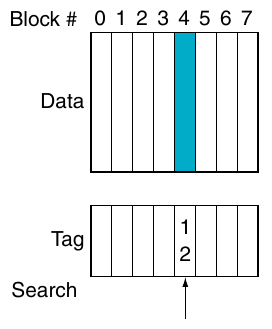
\includegraphics[width=0.25\textwidth]{./figures/1_way_associative.png}
                    \end{minipage}
                  }
                }
              }
              child {
                node {N-way set associative
                  \resizebox{\textwidth}{!}{
                    \begin{minipage}[t]{12cm}
                      \begin{itemize}
                        \item $a$ choices within a set
                        \item All the tags of all the blocks in the set must be searched, becauase a block may be placed in any element of the set
                        \item cache access consists of indexing the appropriate set and then searching the tags of the set
                        \item Each block in the memory maps to a unique set in the cache given by the index field
                        \item Each increase by a factor of $2$ in associativity \alert{doubles the number of blocks per set} and \alert{halves the number of sets}
                        \begin{itemize}
                          \item Accordingly, each factor-of-2 increase in associativity \alert{decreases the size of the index} by $1$ bit and \alert{expands the size of the tag} by $1$ bit
                        \end{itemize}
                        \item $Block\ cache\ address = (Block\ memory\ address)\ modulo\ (\#Sets\ in\ the\ cache)$
                        \item \alert{Size of the tag field:} $32 - (n'-log_2(a) + m + 2) = 32 - (n + m + 2)$ (32-bit address, $n'$ is the number of index bits in a direct-mapped cache)
                        \item $\displaystyle \#Sets = \frac{Cache\ size}{Block\ size \cdot Associativity} = \frac{2^n \cdot 2^m \cdot a}{2^m \cdot a} = 2^n = 2^{n'-log_2(a)} = \frac{2^{n'}}{a}$, so $n$ bits are used for the index
                        \item \alert{Total number of bits:} $\#sets \times associativity \times(block\_size + tag\_size + valid\_field\_size) = a \times \frac{2^{n'}}{a} \times (2^m \times 32 + (32 - (n'-log_2(a) + m + 2)) + 1 ) = a \times 2^n \times ( 2^{m+5} + 31 - n - m)$
                      \item \alert{Associativity:} $\displaystyle \frac{nette\_set\_size}{block\_size} = \frac{\frac{2^n \cdot 2^m \cdot associativity}{2^n}}{2^m}$ (if $n = 32-(m+2)$, then the cache can store as much as the memory region it's responsable for)
                      \end{itemize}
                      \centering
                      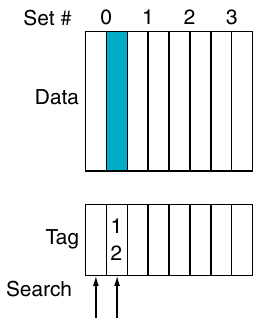
\includegraphics[width=0.25\textwidth, valign=t]{./figures/two_way_associative.png}
                      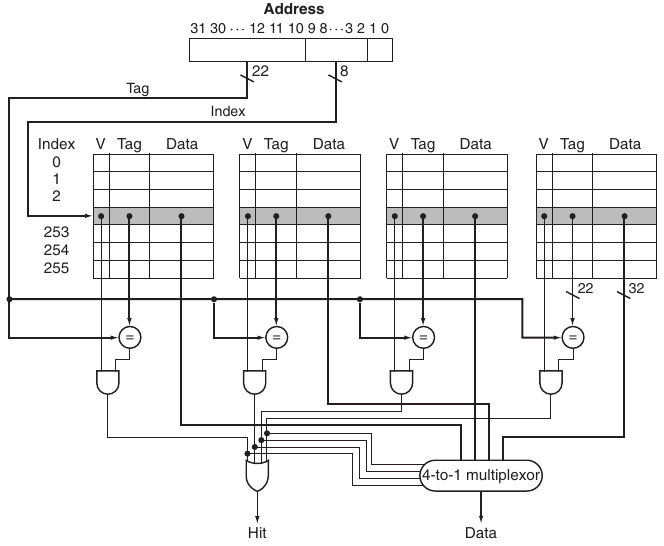
\includegraphics[width=0.5\textwidth, valign=t]{./figures/set_associative_cache.png}
                    \end{minipage}
                  }
                }
              }
              child {
                node {Fully associative
                  \resizebox{\textwidth}{!}{
                    \begin{minipage}[t]{12cm}
                      \begin{itemize}
                        \item Any location
                        \item is an \alert{m-way set-associative cache}, it has one set with $m$ blocks
                        \begin{itemize}
                          \item Thus, there is \alert{no index}
                        % , and the entire address, excluding the block offset, is compared against the tag of every block.
                        \end{itemize}
                        \item \alert{Size of the tag field:} $32 - (m + 2)$ (32-bit address)
                        \item $\displaystyle \#Sets = 1$, $\displaystyle \#Blocks = \frac{Netto\ cache\ size}{Block\ size} = \frac{Netto\ cache\ size}{2^m}$
                        \item \alert{Total number of bits:} $\#blocks \times(block\_size + tag\_size + valid\_field\_size) = \#blocks \times (2^m \times 32 + (32 - (m + 2)) + 1) = \#blocks \times (2^{m+5} + 31 - m)$
                        \item All tags of all the blocks in the cache must be searched, because a block can go anywhere
                        \item To make the search practical, it is done in parallel with a comparator associated with each cache entry. These comparators significantly increase the hardware cost, effectively making fully associative placement practical only for caches with small numbers of blocks
                        \item \alert{Maximum Associativity:} $\displaystyle \frac{nette\_set\_size}{block\_size} = \frac{2^{32-2-m} \cdot 2^m}{2^m}$ (if the cache can store as much as the memory region it's responsable for)
                      \end{itemize}
                      \centering
                      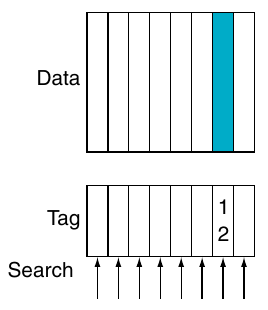
\includegraphics[width=0.25\textwidth]{./figures/fully_associative.png}
                    \end{minipage}
                  }
                }
              }
          }
        }
    };
  \end{scope}
  % ┌───────────────────┐
  % │ Verbindungslinien │
  % └───────────────────┘
  \begin{pgfonlayer}{background}
  \draw [concept connection]
      (commoncasefast) edge (amdahl)
      (branchpredictionbuffer) edge (2bitpredictor)
      (loadusedatahazard) edge (forwarding)
      (datahazardsforbranches) edge (forwarding);
  \end{pgfonlayer}
  % ┌──────────────┐
  % │ Annotationen │
  % └──────────────┘
  % https://tex.stackexchange.com/questions/302976/node-positioning-middle-point-mind-map-connection-bar
  \path (measuringexecutiontime) -- node[annotation, above, align=center, pos=0.01] {Similiar to \textbf{Response Time:} How long it takes to do a task} (ca);
  \path (performance) -- node[annotation, above, align=center, pos=0.01] {Similiar to \textbf{Throughput}: Total work done per time unit (e.g. tasks, transactions\ldots / per hour)} (ca);
  \path (elapsedtime) -- node[annotation, above, align=center, pos=0.01] {Also called \textbf{Wall Clock Time} or \textbf{Real Time}} (ca);
  \path (cputime) -- node[annotation, above, align=center, pos=0.01] {Also called \textbf{User Time}} (ca);
  % \path (branchpredictionbuffer) -- node[annotation, below, align=center, pos=-0.06] {Also called Branch History Table} (ca);
  \path (multicycle) -- node[annotation, above, align=center, pos=0.01] {Optimize space} (ca);
  \path (pipelining) -- node[annotation, above, align=center, pos=0.01] {Optimize time} (ca);
  \node [annotation, below] at (ca.south) {This mindmap is provided without guarantee of correctness and completeness!};
  \end{tikzpicture}
\end{document}


\end{document}
